\documentclass[a4paperpaper,]{article}
\usepackage{lmodern}
\usepackage{amssymb,amsmath}
\usepackage{ifxetex,ifluatex}
\usepackage{fixltx2e} % provides \textsubscript
\ifnum 0\ifxetex 1\fi\ifluatex 1\fi=0 % if pdftex
  % \usepackage[T1]{fontenc}
  % \usepackage[LGRx, T1]{fontenc}
  \usepackage[utf8x]{inputenc}
  % \usepackage[utf8x]{inputenc}
  % \usepackage[greek,english]{babel}
  % \usepackage{CJKutf8}
% \usepackage{textcomp}
  % \usepackage{textgreek}
\else % if luatex or xelatex
  \ifxetex
    \usepackage{mathspec}
  \else
    \usepackage{fontspec}
  \fi
  \defaultfontfeatures{Ligatures=TeX,Scale=MatchLowercase}
\fi
% use upquote if available, for straight quotes in verbatim environments
\IfFileExists{upquote.sty}{\usepackage{upquote}}{}
% use microtype if available
\IfFileExists{microtype.sty}{%
\usepackage{microtype}
\UseMicrotypeSet[protrusion]{basicmath} % disable protrusion for tt fonts
}{}
\usepackage[top=2.54cm, bottom=2.54cm, left=2.4cm, right=2.4cm]{geometry}
\usepackage{hyperref}
\hypersetup{unicode=true,
            pdftitle={Scientific Programming - Assignment 1},
            pdfborder={0 0 0},
            breaklinks=true}
\urlstyle{same}  % don't use monospace font for urls
\usepackage{color}
\usepackage{fancyvrb}
\newcommand{\VerbBar}{|}
\newcommand{\VERB}{\Verb[commandchars=\\\{\}]}
\DefineVerbatimEnvironment{Highlighting}{Verbatim}{commandchars=\\\{\}}
% Add ',fontsize=\small' for more characters per line
\usepackage{framed}
\definecolor{shadecolor}{RGB}{248,248,248}
\newenvironment{Shaded}{\begin{snugshade}}{\end{snugshade}}
\newcommand{\KeywordTok}[1]{\textcolor[rgb]{0.13,0.29,0.53}{\textbf{#1}}}
\newcommand{\DataTypeTok}[1]{\textcolor[rgb]{0.13,0.29,0.53}{#1}}
\newcommand{\DecValTok}[1]{\textcolor[rgb]{0.00,0.00,0.81}{#1}}
\newcommand{\BaseNTok}[1]{\textcolor[rgb]{0.00,0.00,0.81}{#1}}
\newcommand{\FloatTok}[1]{\textcolor[rgb]{0.00,0.00,0.81}{#1}}
\newcommand{\ConstantTok}[1]{\textcolor[rgb]{0.00,0.00,0.00}{#1}}
\newcommand{\CharTok}[1]{\textcolor[rgb]{0.31,0.60,0.02}{#1}}
\newcommand{\SpecialCharTok}[1]{\textcolor[rgb]{0.00,0.00,0.00}{#1}}
\newcommand{\StringTok}[1]{\textcolor[rgb]{0.31,0.60,0.02}{#1}}
\newcommand{\VerbatimStringTok}[1]{\textcolor[rgb]{0.31,0.60,0.02}{#1}}
\newcommand{\SpecialStringTok}[1]{\textcolor[rgb]{0.31,0.60,0.02}{#1}}
\newcommand{\ImportTok}[1]{#1}
\newcommand{\CommentTok}[1]{\textcolor[rgb]{0.56,0.35,0.01}{\textit{#1}}}
\newcommand{\DocumentationTok}[1]{\textcolor[rgb]{0.56,0.35,0.01}{\textbf{\textit{#1}}}}
\newcommand{\AnnotationTok}[1]{\textcolor[rgb]{0.56,0.35,0.01}{\textbf{\textit{#1}}}}
\newcommand{\CommentVarTok}[1]{\textcolor[rgb]{0.56,0.35,0.01}{\textbf{\textit{#1}}}}
\newcommand{\OtherTok}[1]{\textcolor[rgb]{0.56,0.35,0.01}{#1}}
\newcommand{\FunctionTok}[1]{\textcolor[rgb]{0.00,0.00,0.00}{#1}}
\newcommand{\VariableTok}[1]{\textcolor[rgb]{0.00,0.00,0.00}{#1}}
\newcommand{\ControlFlowTok}[1]{\textcolor[rgb]{0.13,0.29,0.53}{\textbf{#1}}}
\newcommand{\OperatorTok}[1]{\textcolor[rgb]{0.81,0.36,0.00}{\textbf{#1}}}
\newcommand{\BuiltInTok}[1]{#1}
\newcommand{\ExtensionTok}[1]{#1}
\newcommand{\PreprocessorTok}[1]{\textcolor[rgb]{0.56,0.35,0.01}{\textit{#1}}}
\newcommand{\AttributeTok}[1]{\textcolor[rgb]{0.77,0.63,0.00}{#1}}
\newcommand{\RegionMarkerTok}[1]{#1}
\newcommand{\InformationTok}[1]{\textcolor[rgb]{0.56,0.35,0.01}{\textbf{\textit{#1}}}}
\newcommand{\WarningTok}[1]{\textcolor[rgb]{0.56,0.35,0.01}{\textbf{\textit{#1}}}}
\newcommand{\AlertTok}[1]{\textcolor[rgb]{0.94,0.16,0.16}{#1}}
\newcommand{\ErrorTok}[1]{\textcolor[rgb]{0.64,0.00,0.00}{\textbf{#1}}}
\newcommand{\NormalTok}[1]{#1}
\usepackage{longtable,booktabs}
\usepackage{graphicx,grffile}
\makeatletter
\def\maxwidth{\ifdim\Gin@nat@width>\linewidth\linewidth\else\Gin@nat@width\fi}
\def\maxheight{\ifdim\Gin@nat@height>\textheight\textheight\else\Gin@nat@height\fi}
\makeatother
% Scale images if necessary, so that they will not overflow the page
% margins by default, and it is still possible to overwrite the defaults
% using explicit options in \includegraphics[width, height, ...]{}
\setkeys{Gin}{width=\maxwidth,height=\maxheight,keepaspectratio}
\IfFileExists{parskip.sty}{%
\usepackage{parskip}
}{% else
\setlength{\parindent}{0pt}
\setlength{\parskip}{6pt plus 2pt minus 1pt}
}
\setlength{\emergencystretch}{3em}  % prevent overfull lines
\providecommand{\tightlist}{%
  \setlength{\itemsep}{0pt}\setlength{\parskip}{0pt}}
\setcounter{secnumdepth}{5}
% Redefines (sub)paragraphs to behave more like sections
\ifx\paragraph\undefined\else
\let\oldparagraph\paragraph
\renewcommand{\paragraph}[1]{\oldparagraph{#1}\mbox{}}
\fi
\ifx\subparagraph\undefined\else
\let\oldsubparagraph\subparagraph
\renewcommand{\subparagraph}[1]{\oldsubparagraph{#1}\mbox{}}
\fi

%%% Use protect on footnotes to avoid problems with footnotes in titles
\let\rmarkdownfootnote\footnote%
\def\footnote{\protect\rmarkdownfootnote}

%%% Change title format to be more compact
\usepackage{titling}

% Create subtitle command for use in maketitle
\newcommand{\subtitle}[1]{
  \posttitle{
    \begin{center}\large#1\end{center}
    }
}

\setlength{\droptitle}{-2em}
  \title{Scientific Programming - Assignment 1}
  \pretitle{\vspace{\droptitle}\centering\huge}
  \posttitle{\par}
  \author{}
  \preauthor{}\postauthor{}
  \date{}
  \predate{}\postdate{}


\begin{document}
\maketitle

{
\setcounter{tocdepth}{3}
\tableofcontents
}
\section{What is this?}\label{what-is-this}

This document is the work of \textbf{a random student}, completed as an
assignment for the Scientific Programming module as part of MPhil
Computational Biology at DAMTP.

\section{Results:}\label{results}

\subsection{Analysing Words}\label{analysing-words}

\subsubsection{Q: How many unique words are there (ignoring
cases)?}\label{q-how-many-unique-words-are-there-ignoring-cases}

\begin{verbatim}
## A: 97723
\end{verbatim}

\subsubsection{Q: How many words contain an
apostrophe(')?}\label{q-how-many-words-contain-an-apostrophe}

\begin{longtable}[]{@{}l@{}}
\toprule
words.match\_idx.\tabularnewline
\midrule
\endhead
A'S\tabularnewline
AA'S\tabularnewline
AB'S\tabularnewline
ABM'S\tabularnewline
AC'S\tabularnewline
ACTH'S\tabularnewline
AI'S\tabularnewline
AIDS'S\tabularnewline
AM'S\tabularnewline
AOL'S\tabularnewline
\bottomrule
\end{longtable}

\begin{verbatim}
## A: 25751  
## 71972 words left after filtering
\end{verbatim}

\subsubsection{\texorpdfstring{Q: How many words contain non-ASCII
chars? Save the filtered words as
`database'.}{Q: How many words contain non-ASCII chars? Save the filtered words as database.}}\label{q-how-many-words-contain-non-ascii-chars-save-the-filtered-words-as-database.}

\begin{longtable}[]{@{}l@{}}
\toprule
words.match\_idx.\tabularnewline
\midrule
\endhead
ASUNCIÓN\tabularnewline
ATATÜRK\tabularnewline
BARTÓK\tabularnewline
BOGOTÁ\tabularnewline
BOÖTES\tabularnewline
BUÑUEL\tabularnewline
CONCEPCIÓN\tabularnewline
DVORÁK\tabularnewline
DÜRER\tabularnewline
DÜSSELDORF\tabularnewline
\bottomrule
\end{longtable}

\begin{verbatim}
## A: 159  
## 71813 words left after filtering, saved to "words_data"
\end{verbatim}

\subsubsection{Q: Find all the words as the two related form XOG and
XOGUE, for example CATALOG and
CATALOGUE.}\label{q-find-all-the-words-as-the-two-related-form-xog-and-xogue-for-example-catalog-and-catalogue.}

\begin{verbatim}
## 10 pairs of words were found to conform "XOG"->"XOGUE" projection
\end{verbatim}

\begin{longtable}[]{@{}ll@{}}
\caption{Showing best 10 hits below:}\tabularnewline
\toprule
XOG & XOGUE\tabularnewline
\midrule
\endfirsthead
\toprule
XOG & XOGUE\tabularnewline
\midrule
\endhead
ANALOG & ANALOGUE\tabularnewline
CATALOG & CATALOGUE\tabularnewline
DEMAGOG & DEMAGOGUE\tabularnewline
DIALOG & DIALOGUE\tabularnewline
EPILOG & EPILOGUE\tabularnewline
MONOLOG & MONOLOGUE\tabularnewline
PEDAGOG & PEDAGOGUE\tabularnewline
PROLOG & PROLOGUE\tabularnewline
SYNAGOG & SYNAGOGUE\tabularnewline
TRAVELOG & TRAVELOGUE\tabularnewline
\bottomrule
\end{longtable}

\subsubsection{\texorpdfstring{Q: Load scrabble scores for the alphabet
from ``scarabble.txt'', store to
``scores''}{Q: Load scrabble scores for the alphabet from scarabble.txt, store to scores}}\label{q-load-scrabble-scores-for-the-alphabet-from-scarabble.txt-store-to-scores}

\begin{longtable}[]{@{}ll@{}}
\caption{Showing best 10 hits below:}\tabularnewline
\toprule
& scores\tabularnewline
\midrule
\endfirsthead
\toprule
& scores\tabularnewline
\midrule
\endhead
Q & 10\tabularnewline
Z & 10\tabularnewline
J & 8\tabularnewline
X & 8\tabularnewline
K & 5\tabularnewline
F & 4\tabularnewline
H & 4\tabularnewline
V & 4\tabularnewline
W & 4\tabularnewline
Y & 4\tabularnewline
\bottomrule
\end{longtable}

\subsubsection{Q: Compute the scrabble score for each word in the
database. Plot the distribution of scores. What is the highest-scoring
word}\label{q-compute-the-scrabble-score-for-each-word-in-the-database.-plot-the-distribution-of-scores.-what-is-the-highest-scoring-word}

\emph{(Summation of score is assumed)}

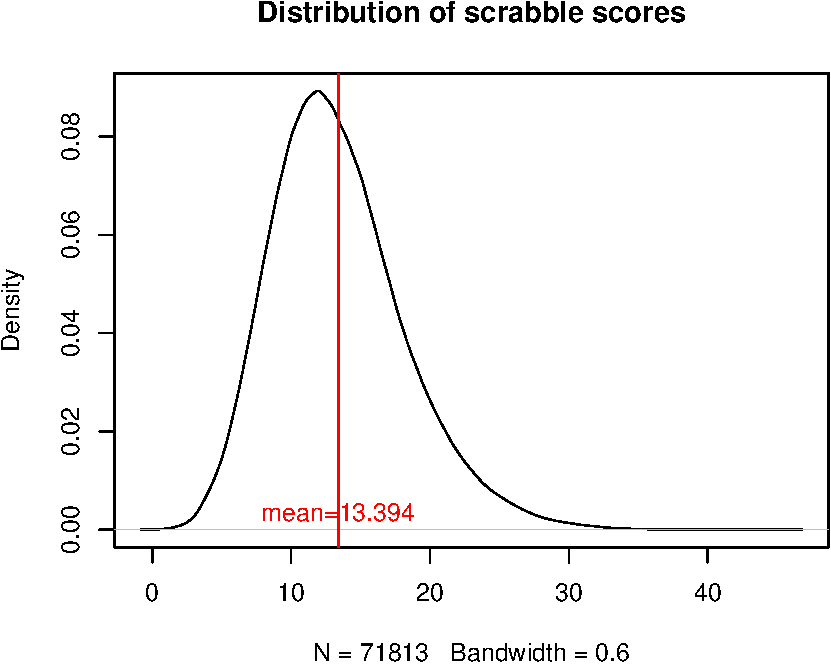
\includegraphics{index_files/figure-latex/word6-1.pdf}

\begin{verbatim}
## Highest score is achieved by: PIZZAZZ , Score: 45
\end{verbatim}

\subsubsection{Q: Find all words W where both W and its reverse
complement are both in the
database.}\label{q-find-all-words-w-where-both-w-and-its-reverse-complement-are-both-in-the-database.}

\begin{verbatim}
## We found 68 entries, out of which 16 are reverse-complement to themselves , Showing longest 10 entries
\end{verbatim}

\begin{longtable}[]{@{}ll@{}}
\caption{Showing best 10 hits below:}\tabularnewline
\toprule
smaller\_word & larger\_word\tabularnewline
\midrule
\endfirsthead
\toprule
smaller\_word & larger\_word\tabularnewline
\midrule
\endhead
BOORISH & SHRILLY\tabularnewline
HOVELS & HOVELS\tabularnewline
WIZARD & WIZARD\tabularnewline
BOORS & HILLY\tabularnewline
HOOFS & HULLS\tabularnewline
ARIZ & ARIZ\tabularnewline
BEVY & BEVY\tabularnewline
BIRD & WIRY\tabularnewline
BOIL & ORLY\tabularnewline
GILL & OORT\tabularnewline
\bottomrule
\end{longtable}

\subsubsection{\texorpdfstring{Q: Using ``F A L U Y P L N I'', how many
words of four or more letters can you find that are in the database AND
all contain the letter
A?}{Q: Using F A L U Y P L N I, how many words of four or more letters can you find that are in the database AND all contain the letter A?}}\label{q-using-f-a-l-u-y-p-l-n-i-how-many-words-of-four-or-more-letters-can-you-find-that-are-in-the-database-and-all-contain-the-letter-a}

\begin{verbatim}
## We found 39 hits according to query "LLFAUYPNI" in "words_data"", 
##  (Option: min_len=4, special=A).
\end{verbatim}

\begin{longtable}[]{@{}llll@{}}
\caption{Showing best 20 hits below:}\tabularnewline
\toprule
& words\_res & words\_len & words\_score\tabularnewline
\midrule
\endfirsthead
\toprule
& words\_res & words\_len & words\_score\tabularnewline
\midrule
\endhead
44850 & PAINFULLY & 9 & 9\tabularnewline
23582 & FINALLY & 7 & 7\tabularnewline
44840 & PAILFUL & 7 & 7\tabularnewline
44847 & PAINFUL & 7 & 7\tabularnewline
47295 & PLAINLY & 7 & 7\tabularnewline
47419 & PLAYFUL & 7 & 7\tabularnewline
25465 & FULANI & 6 & 6\tabularnewline
23572 & FINAL & 5 & 5\tabularnewline
23863 & FLAIL & 5 & 5\tabularnewline
32408 & INLAY & 5 & 5\tabularnewline
45662 & PAULI & 5 & 5\tabularnewline
46955 & PILAF & 5 & 5\tabularnewline
46963 & PILAU & 5 & 5\tabularnewline
47289 & PLAIN & 5 & 5\tabularnewline
1332 & AINU & 4 & 4\tabularnewline
1705 & ALLY & 4 & 4\tabularnewline
22746 & FAIL & 4 & 4\tabularnewline
22753 & FAIN & 4 & 4\tabularnewline
22807 & FALL & 4 & 4\tabularnewline
23063 & FAUN & 4 & 4\tabularnewline
\bottomrule
\end{longtable}

\subsection{Examination Marking}\label{examination-marking}

\subsubsection{Importing and Scoring:}\label{importing-and-scoring}

\begin{verbatim}
## [DEBUG]:There are 100 questions from file:crib.dat
\end{verbatim}

\begin{longtable}[]{@{}rrrlr@{}}
\caption{Result of 12 students in this exam, sorted by percent score in
descending order}\tabularnewline
\toprule
student\_idx & score & percent & grade & rank\tabularnewline
\midrule
\endfirsthead
\toprule
student\_idx & score & percent & grade & rank\tabularnewline
\midrule
\endhead
7 & 29 & 96 & A & 1.0\tabularnewline
2 & 24 & 80 & A & 2.0\tabularnewline
6 & 23 & 76 & A & 3.0\tabularnewline
9 & 22 & 73 & A & 4.0\tabularnewline
5 & 20 & 66 & B & 5.0\tabularnewline
1 & 19 & 63 & B & 6.0\tabularnewline
12 & 18 & 60 & B & 7.0\tabularnewline
4 & 17 & 56 & C & 8.5\tabularnewline
10 & 17 & 56 & C & 8.5\tabularnewline
3 & 14 & 46 & D & 10.0\tabularnewline
11 & 9 & 30 & F & 11.0\tabularnewline
8 & 7 & 23 & F & 12.0\tabularnewline
\bottomrule
\end{longtable}

\begin{verbatim}
## Stats were calculated for the rounded percent score for 12 students in the exam
\end{verbatim}

\begin{verbatim}
##    Min. 1st Qu.  Median    Mean 3rd Qu.    Max. 
##   23.00   53.50   61.50   60.42   73.75   96.00
\end{verbatim}

\subsubsection{Detecting cheating}\label{detecting-cheating}

\paragraph{Naive approach}\label{naive-approach}

We define cheat index between two students, as the number of questions
with a same answer, divided by the product of overlapped questions. \[ 
I_{cheat}^{(a,b)} = 
  {\sum_{i}{\delta_{A_i^a,A_i^b} }
  \over
  {\sum_{i}{\delta_{Q_i^a,Q_i^b} } } 
  }
\] where \(a,b\) denotes index of students, \(A_i^a\) denotes answer to
question i by student a, \(Q_i^a\) denotes whether question i is
answered by student a, \(\delta_{x,y}\) defined as

\[ 
\delta_{x,y} = \left\{
  \begin{array}{ll}
            0 & x \neq y \\
            1 & x = y
  \end{array}
\right.
\] Specifically, if any of the \(A_i^a,A_i^b\) is undefined, then
\(\delta_{A_i^a,A_i^b} = 0\).

Normalisation against overlapped questions count is important, because
students can give the same answer by chance even without cheating.
However, the calculated cheat index appear to follow a normal
distribution, without a significant outlier. (See Figure
\ref{fig:exam_naive} )

\begin{figure}
\centering
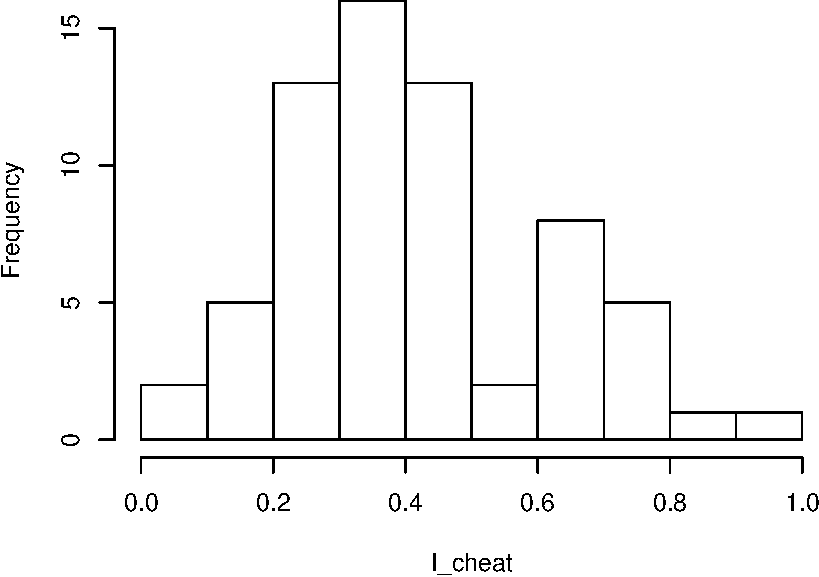
\includegraphics{index_files/figure-latex/exam_naive-1.pdf}
\caption{\label{fig:exam_naive} Distribution of \(I_{cheat}\)}
\end{figure}

\paragraph{Diagnostic approach}\label{diagnostic-approach}

To obtain a more solid result, we plotted the numerator of \(I_{cheat}\)
against its denominator, allowing for a careful examination of the
relation between overlapped answers and overlapped questions. We then
fitted this relation with linear regression
\(N_{answer} = a\cdot N_{question} + \epsilon\), estimated the standard
deviation of the resultant residual \(\sigma(\epsilon)\). The estimated
standard deviation is then used to normalise the residual distribution,
and to calculate the corresponding P-value, indicating our confidence to
reject the null hypothesis that the point is sampled from this
distribution (Figure \ref{fig:exam_diag}).

From a visual inspection, point 15 comparison is obviously an outlier to
the other clustered points. The normalised stats can be found at Table
\ref{tab:exam_diag}. We conclude student 2 and student 6 (graded A and B
respectively) are highly likely to have cheated (with a 99.99994\%
confidence), giving identical answers to all 27 quesions that were
allocated to both of them.

We also detected other students sharing a large number of answers, but
associated with less significant z-score and are subject to further
discussion. , we need to account for the fact that some questions are so
easy that every student get it right, thus giving the same answer. The
difficulty can be measured with Shannon entropy, and can be used to
score the observed conincidence, instead of simple scoring by counting.

\textbf{We refrain from a thorough treatment given the size limit of
this report.}

\begin{figure}
\centering
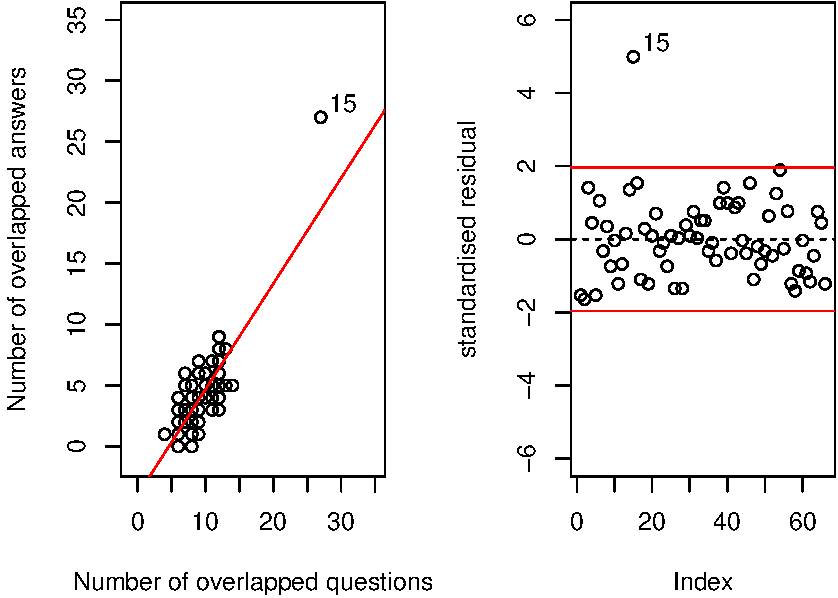
\includegraphics{index_files/figure-latex/exam_diag-1.pdf}
\caption{\label{fig:exam_diag} Diagnostic plots for finding the
outlier/cheater\newline (Using 95.000 \% confidence (2 tailed) as
threshold)}
\end{figure}

\begin{longtable}[]{@{}lrlrlrrr@{}}
\caption{\label{tab:exam_diag}Showing best 10 hits
below:}\tabularnewline
\toprule
& stud\_A & grad & stud\_B & grad.1 & ques\_same & ans\_same &
Confidence\_to\_reject\_NULL\tabularnewline
\midrule
\endfirsthead
\toprule
& stud\_A & grad & stud\_B & grad.1 & ques\_same & ans\_same &
Confidence\_to\_reject\_NULL\tabularnewline
\midrule
\endhead
15 & 2 & A & 6 & B & 27 & 27 & 0.9999994\tabularnewline
54 & 7 & B & 10 & D & 7 & 6 & 0.9415630\tabularnewline
16 & 2 & A & 7 & B & 9 & 7 & 0.8743686\tabularnewline
46 & 6 & B & 7 & B & 9 & 7 & 0.8743686\tabularnewline
3 & 1 & A & 4 & A & 7 & 5 & 0.8417347\tabularnewline
39 & 5 & B & 6 & B & 7 & 5 & 0.8417347\tabularnewline
14 & 2 & A & 5 & B & 6 & 4 & 0.8240609\tabularnewline
53 & 7 & B & 9 & C & 12 & 9 & 0.7882032\tabularnewline
6 & 1 & A & 7 & B & 9 & 6 & 0.7073157\tabularnewline
38 & 4 & A & 12 & F & 8 & 5 & 0.6779376\tabularnewline
\bottomrule
\end{longtable}

\subsection{\texorpdfstring{Treatment to Chapter 10 from ``Dynamical
Models in Biology'' {[}1{]}
\label{sec:DMB}}{Treatment to Chapter 10 from Dynamical Models in Biology {[}1{]} }}\label{treatment-to-chapter-10-from-dynamical-models-in-biology-ellner2011}

\subsubsection{Introduction}\label{introduction}

In ecology, people study population growth from a spatial perspective.
This could be done by discretising space into a lattice of cells, and
specify a recursion formula to account for both the constitutive
geometric growth the spatial dispersal. Here we consider a such model
from {[}1{]} where the population \(N(s, t)\) is a function of both
space \(s\) and time \(t\). Two phenomena are included in this model:

\pagebreak[4]

\paragraph{Geometric growth}\label{geometric-growth}

\begin{enumerate}
\def\labelenumi{(\arabic{enumi})}
\tightlist
\item
  \[
  \begin{aligned}
  M(s,t) = \lambda(s) \cdot  N(s,t) 
  \end{aligned}
  \]
\end{enumerate}

where M is an intermediate variable to be transformed back into N.

\paragraph{Spatial dispersal}\label{spatial-dispersal}

\begin{enumerate}
\def\labelenumi{(\arabic{enumi})}
\setcounter{enumi}{1}
\tightlist
\item
  \[
  N(s,t+1) = \begin{bmatrix}M(s-1,t),& M(s,t),&M(s+1,t)\end{bmatrix} \cdot { \begin{bmatrix}d\\ 1-2d\\ d \end{bmatrix} }
  \]
\end{enumerate}

This is equivalent to convolve signal \(M_{t}(s)\) with filter \(D(i)\)
\[
N_{t+1}(s) = \sum_{i } M_{t}(s+i) \cdot  D(i) 
\]

where \[
\begin{array}{ll}
D(i) = \left\{
  \begin{array}{ll}
            d & i \in \{- 1,+1\}\\
            1-2d & i= 0 \\
            0 & for~other~i
  \end{array}
\right.
\end{array}
\]

Importantly, this filter implies a weighted sum of nearest neighbors,
for we have \[
\sum_i{D(i)} = (d) + (1-2d) + (d) = 1
\]

this is clearer if we set \(K = s+i\) to obtain

\begin{enumerate}
\def\labelenumi{(\arabic{enumi})}
\setcounter{enumi}{2}
\tightlist
\item
  \[
  \begin{aligned}
  \sum_{s}{N_{t+1}(s)} &= \sum_{s}{ \left( \sum_{i } M_{t}(s+i) \cdot  D(i) \right) } \\
                   &= \sum_{s}  \left( \sum_{K} M_{t}(K) \cdot  D(K-s)  \right)  \\
                   &= \sum_{K}  \left( M_t(K) \cdot  \sum_{s}{D(K-s)}   \right) \\
                   &= \sum_{K}M_t(K) \cdot  1 \\
  \sum_{s}{N_{t+1}(s)} &= \sum_{K}M_t(K)
  \end{aligned} 
  \]
\end{enumerate}

,which implies application of the spatial dispersal rule perserves the
overall population. Since we are running finite simulation on
\(s \in [1,L]\) (\([a,b]\) means integers \(a,a+1,...,b\) if not
otherwise specified), special treatment is required at border, namely
\(M(s-1)_{|s = 0}= M(s)_{|s = 0}\) and \(M(s+1)_{|s = L}=M(s)_{|s = L}\)
where \(s-1,s+1\) are undefined. It's easy to verify eq(3) stays true
for this finite \(\{s\}\) under such treatment,by constructing an
infinite array of \([1,L]\) and exploiting its symmetry.

\subsubsection{Introducing tools for
visualising}\label{introducing-tools-for-visualising}

Given that spatial dispersal is merely a re-distribution of existing
population, we reason it is merely adding a twist to the constitutive
geometric growth process, as described by eq(1). The existence of
dispersal ensures

\[
N_{t+1}(s) \neq \lambda(s) \cdot  N_{t}(s) 
\]

, which will be true if geometric growth is the only process.
Nevertheless, we can still exploit this formalism to describe the growth
process, by defining

\[
N_{t+1}(s) = \mu_t(s) \cdot N_{t}(s)  \\
\mu_t(s)   =  \frac{N_{t+1}(s)}{N_{t}(s)}
\]

However, \(\mu_t(s)\) is undefined if \(N_t(s)=0\). To resolve this
issue,we transform the \(N(s)\) with a modified version of lograthmic
function eq(4), use of which also allows comparison between population
across different scales.

\begin{enumerate}
\def\labelenumi{(\arabic{enumi})}
\setcounter{enumi}{3}
\tightlist
\item
  \[
  f(x) = \log_{10}(1+10\cdot x) 
  \]
\end{enumerate}

and the logarithm of \(\mu_t(s)\) is estimated with \(\nu_t(s)\)

\begin{enumerate}
\def\labelenumi{(\arabic{enumi})}
\setcounter{enumi}{4}
\tightlist
\item
  \[
  \begin{aligned}
    log_{10}(\mu_t(s)) &= \log_{10}(\frac{N_{t+1}(s)}{N_{t}(s)})  \\
                   &= \log_{10}(N_{t+1}(s)) - \log_{10}(N_{t}(s)) \\
                   &= \log_{10}(10\cdot N_{t+1}(s)) - \log_{10}(10 \cdot N_{t}(s)) \\
                   &\sim \log_{10}(1+10\cdot N_{t+1}(s)) - \log_{10}(1+10\cdot N_{t}(s))\\
          \nu_t(s) &= f(N_{t+1}(s)) - f(N_{t}(s))
  \end{aligned}
  \]
\end{enumerate}

To illustrate, we setup a simulation with initial condition and graph
\(f(N_t(s))\), \(\nu_t(s)\), \(f(\sum_s(N_t(s))\) accordingly for
\(t \in [1,50]\):

\begin{enumerate}
\def\labelenumi{(\arabic{enumi})}
\setcounter{enumi}{5}
\tightlist
\item
  \[
  \left\{
    \begin{aligned}
  & N_1(s)=5, s \in [1,20] \\
  & d = 0.1 \\
  & \lambda(s)  = 
  \left\{
  \begin{aligned}
  0.9 &~~~~ s \in [1,10]\\ 
  1.1 &~~~~ s \in [11,20]
  \end{aligned}\right. \\
    \end{aligned}
  \right.
  \]
\end{enumerate}

\begin{figure}
\centering
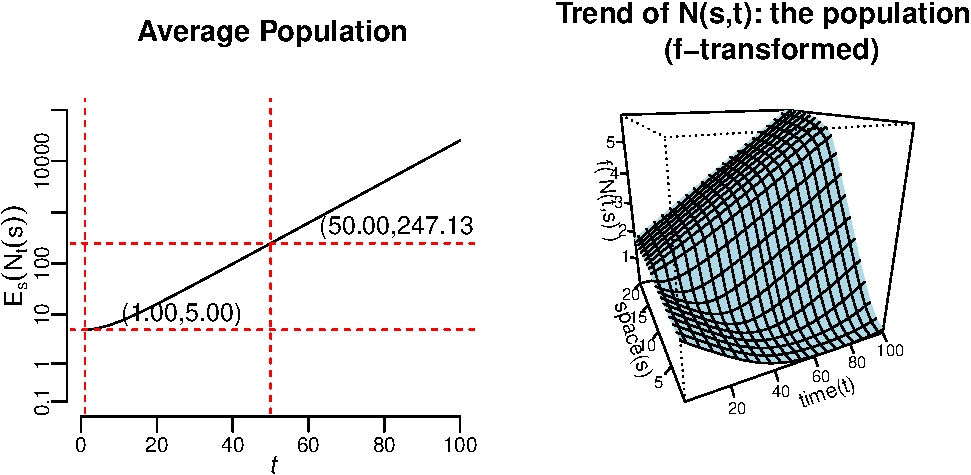
\includegraphics{index_files/figure-latex/DMB_log-1.pdf}
\caption{\label{fig:DMB_log} Simple visualisation without taking
differential}
\end{figure}

\begin{figure}
\centering
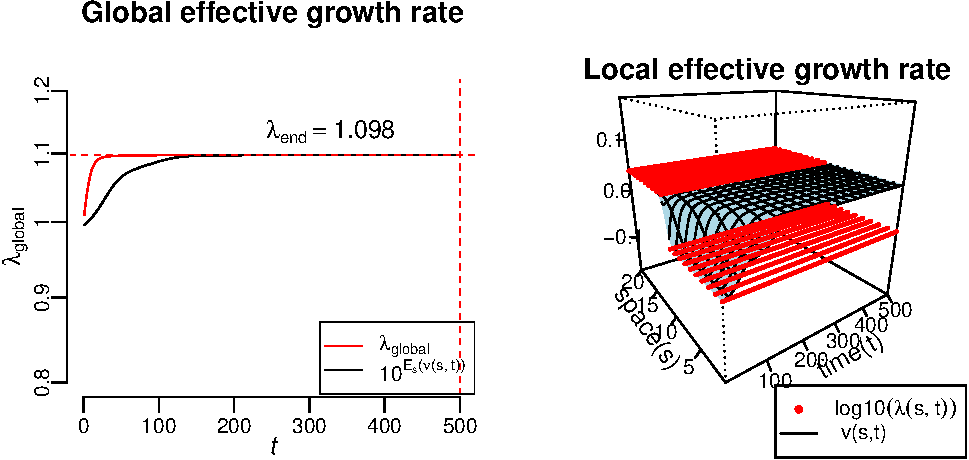
\includegraphics{index_files/figure-latex/DMB_logdiff-1.pdf}
\caption{\label{fig:DMB_logdiff} Visualisation after taking differential
w.r.t. time}
\end{figure}

The obseved linear trends also justify our use of \(\nu(s,t)\) eq(5),
which essantially results from the application of abackward difference
operator along the time axis, in other words: \[
\nu_t(s) = D_t(N_t(s))
\] where \(D_t\) is the backward difference operator so that \[
D_t(f_t)=f_{t}-f_{t-1}
\]

\paragraph{\texorpdfstring{The steady global growth rate
\(\lambda_{end}\)}{The steady global growth rate \textbackslash{}lambda\_\{end\}}}\label{the-steady-global-growth-rate-lambda_end}

\newcommand{\lend}{1.098}

The linear tail at \(t\rightarrow\infty\) indicates the total population
settles into a steady growth state, namely
\(\lambda_{global}(t) = \frac{E_s(N_{t}(s))}{E_s(N_{t-1}(s))} \rightarrow \lend\)
and \(10^{E_s(\nu_t(s))} \rightarrow \lend\) as \(t\rightarrow\infty\)
(see figure \ref{fig:DMB_logdiff}). Define: \[
\lambda_{end} = \lim_{t\rightarrow\infty} \lambda_{global}(t)
\] Given our finite simulation size, we can only approximate this limit
by extending the simulation time. Throughout the analysis, we record
\(\lambda_{end} = E_t[\lambda_{global}(t)]\) from 20 consecutive
\(\lambda_{global}(t)\) if
\(\sigma_t[\log_{10}(\lambda_{global}(t))]<10^{-5}\).

Definition of \(\lambda_{end}\) is also justified by the observation
that \(\sigma_s(\nu(s))\rightarrow 0\) as \(t\rightarrow\infty\), that
is, \(\nu(s)\) freezes into a constant independent of the position:
\(\nu(s)=\nu_{end}\). Because \(\nu_t(s)\) approximates \(\mu_t(s)\), we
assume \(\mu_t(s)\) is constant, aka:

\[
\begin{aligned}
  \nu_t(s)  &= \nu_{end}, but ~~
  \nu_t(s) \sim \mu_t(s) \\
  \mu_t(s)  &= \mu_{end} \\
\end{aligned}
\]

Then by definition of \(\mu_t(s)\), we can deduce that global population
also grows at a constant rate:

\[
\begin{aligned}
  \mu_{end} &= \log_{10}( \frac{ N_{t+1}(s) }{N_{t}(s)} ) \\
  10^{\mu_{end}} &= \frac{N_{t+1}(s)}{N_{t}(s)} \\
  E_s \left[ {N_{t+1}(s)} \right.] &= E_s  \left[ {10^{\mu_{end}} \cdot N_t(s)} \right.] \\
  E_s \left[ {N_{t+1}(s)} \right.] &=  {10^{\mu_{end}} E_s[ N_t(s)} ] \\
  \log_{10}\left( \frac{E_s[N_{t+1}(s)]}{E_s[N_t(s)]} \right) &=\mu_{end} \\
  \lambda_{end} &= \mu_{end}
\end{aligned}
\]

\subsubsection{\texorpdfstring{Factors that affect
\(\lambda_{end}\)}{Factors that affect \textbackslash{}lambda\_\{end\}}}\label{factors-that-affect-lambda_end}

\emph{Note: We make the empirical assumption that \(\lambda_{end}\) is
independent of \(N_1(s)\) (see appendix figure \ref{fig:vis__N1})}

We then ask what factors determine \(\lambda_{end}\). We know it is not
a simple average of \(\lambda(s)\) since
\(E_s(\lambda(s))=1.0\neq \lend = \lambda_{end}\) from eq(6).

\paragraph{Limit case: No spatial
dispersal}\label{limit-case-no-spatial-dispersal}

In the limit case without dispersal (\(d = 0.0\)), we anticipate the
global growth to be dominated by the patch with the greatest
\(\lambda(s)\), whose population would eventually take over given a
sufficiently long period. Formally:

\begin{enumerate}
\def\labelenumi{(\arabic{enumi})}
\setcounter{enumi}{6}
\tightlist
\item
  \[
  \lambda_{end} = max_s(\lambda(s)), when ~d=0.00 
  \]
\end{enumerate}

Although this no longer holds for \(d>0\), we can still anticipate a
proportionality that \(\lambda_{end}= A \cdot max_s(\lambda(s))\), where
factor \(A\) is determined from spatial configuration \(\lambda(s)\). In
other words, the equivalent \(max_s\) operator becomes more complex
because of effect of spatial configuration on cluster growth.

To understand this effect, we keep the magitude of \(\lambda(s)\)
unchanged, but shuffle it spatially instead. We observe variation in
\(\lambda_{end}\) under such shuffling and attempted some modelling (See
\ref{sec:prediction}). We give a brief analysis here before attempting
the actual statistical test.

\paragraph{Effect of the reflective
edge}\label{effect-of-the-reflective-edge}

Consider an edged cluster of good patches \(s_{good}\in[1,8]\) of length
8 on a strip \(\{s\}=[1,20]\) of length 20, where
\(\lambda(s)= \lambda_{good} = 1.1\). If we reflect the whole strip onto
\(\{s\}=[-19,0]\), so that \(\lambda(a-0.5)=\lambda(-a-0.5)\) and
\(N_t(a-0.5)=N_t(-a-0.5)\), then the spatial dispersal eq(2) is
apparently restored in \(s\in[0,1]\), because
\(M_t(0) = \lambda_t(0)\cdot N_t(0) = \lambda_t(1)\cdot N_t(1)=M_t(1)\)

We run a simulation to confirm edge cluster of length 8 on a strip of
length 20 give a same \(\lambda_{end}\) as a central cluster of length
16 on a strip of length 40. (See figure \ref{fig:reflect_sep}). Given
the identical \(\lambda_{global}(t)\), we conclude an edged cluster is
equivalent to a non-edged(central) cluster of a doubled length.

\begin{figure}
\centering
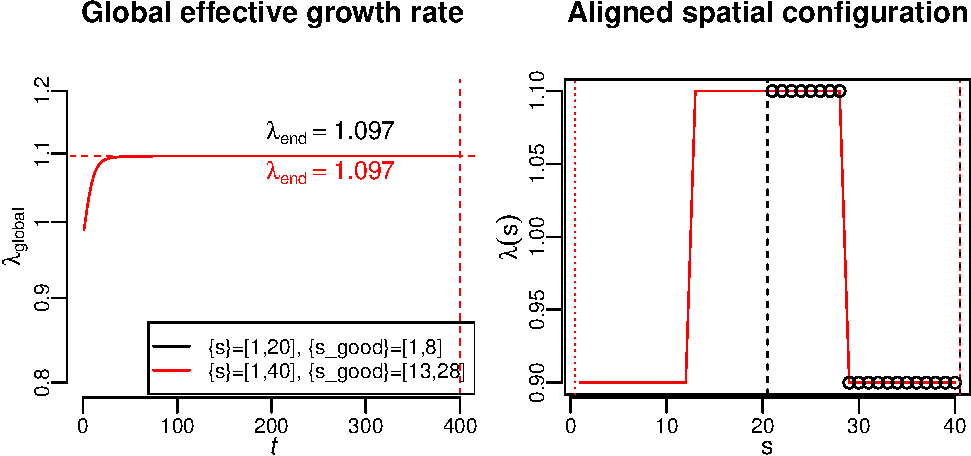
\includegraphics{index_files/figure-latex/reflect_sep-1.pdf}
\caption{\label{fig:reflect_sep} Left: \(\lambda_{end}\) stays invariant
under reflection operation; \newline Right: dotted-line indicates edge
of \{s\}}
\end{figure}

\paragraph{\texorpdfstring{Collective growth of closely separated
clusters
\label{sec:collect}}{Collective growth of closely separated clusters }}\label{collective-growth-of-closely-separated-clusters}

If we do the same reflective operation with a good cluster separated by
\(k\) bad patches from the edge, then we shall obtain central clusters
separated by \(K=2k\) bad patches, which is a subcase of
\(K\in [0,\infty]\). We then measure \(\lambda_{end}\) for
\(K\in[0,10]\), for equally sized unedged clusters on a strip of length
100, with total number of good patches (\(L_{good}=|\{s_{good}\}|\))
that are power of 2. Use of central clusters avoids confounding with the
edge reflection issue. We use \(\lambda_{good}=1.2\) for better
resolution.

Results (figure \ref{fig:vis__K} left) show that at small separations,
growth of two small clusters enhance each other and can be collectively
treated as a cluster of larger size. But this enhancement decays very
quickly as spearation increases, seemingly at an exponential rate. At
large separations, there is so little enhancement that \(\lambda_{end}\)
is same as that of a single cluster. By analogy to eq(7), we assert
\(\lambda_{end}\) is dominated by the largest cluster for sufficiently
large \(K\).

\begin{figure}
\centering
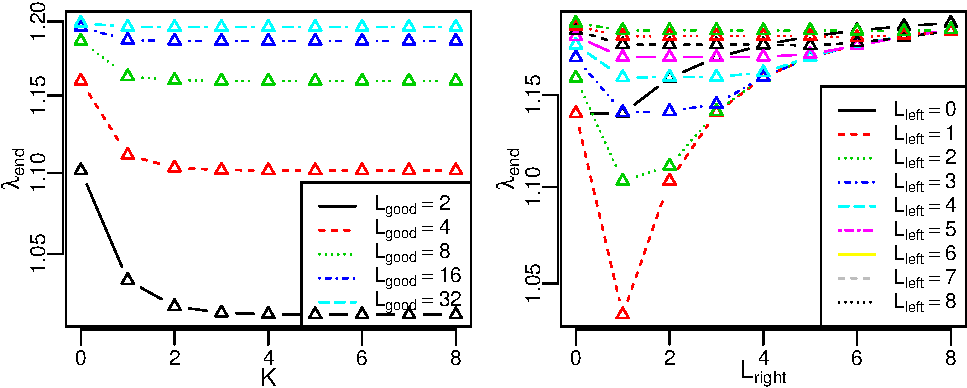
\includegraphics{index_files/figure-latex/vis__lend_K_dp1-1.pdf}
\caption{\label{fig:vis__K} Left: Equally sized clusters at different
separation. Right: Unequally sized clusters at \(K = 1\)}
\end{figure}

To further understand the effect of enhancement at small separations, we
simulate \(K = 1\) cases for unequally-sized clusters. Two clusters are
placed in the center of a strip of length 400. Combinations of cluster
sizes \((L_{left},L_{right})\) of \((0,0)\sim (8,8)\) are considered
(figure \ref{fig:vis__K} right). To our surprise, big cluster receives
impairment rather than enhancement from a smaller cluster. In other
words, a small cluster is more capable of slowing down the larger
cluster than mere bad patches, counter-intuitively. In summary,
collective growth at \(K = 1\) is more like an average of two clusters.
Because of its complexity, this effect is excluded from
\ref{sec:prediction}

\subsubsection{\texorpdfstring{Predict \(\lambda_{end}\) from maximal
cluster size
\label{sec:prediction}}{Predict \textbackslash{}lambda\_\{end\} from maximal cluster size }}\label{predict-lambda_end-from-maximal-cluster-size}

\newcommand{\pvalue}{$2.2\times 10^{-16}$}

Because the \(\lambda_{end}\) from two equally-sized clusters is well
approximated with that from a single cluster for \(K > 1\), we reason
the biggest cluster (\(max(cluster\_size)\)) should dominate
\(\lambda_{end}\). To test this hypothesis, we sampled random spatial
configurations at \(L = 80\), \(L_{good} = 30\), \(\lambda_{good}=1.2\),
\(\lambda_{bad}=0.8\), \(d=0.1\).This is done by taking a random
permutation of length 80 and rearrange the patches accordingly, so that
each permutation is equally likely to be sampled. From (figure
\ref{fig:vis__max_cluster}), \(max(cluster\_size)\) seems to predict the
average \(\lambda_{end}\) accurately, although the exact value varies
for each configuration. This is confirmed with an ANCOVA analysis (P
\textless{} \pvalue). On a sidenote, \(max(cluster\_size)\) itself
follows a non-uniform distribution, with 3,4,5 being the most popular
values. We conclude that maximal cluster is a good predictor of
\(\lambda_{end}\), and that \(\lambda_{end}\) is indeed dominated by the
biggest cluster, though subject to correction from an account of
interaction between closely separated clusters (see \ref{sec:collect})

\begin{verbatim}
## Loading required package: grid
\end{verbatim}

\begin{figure}
\centering
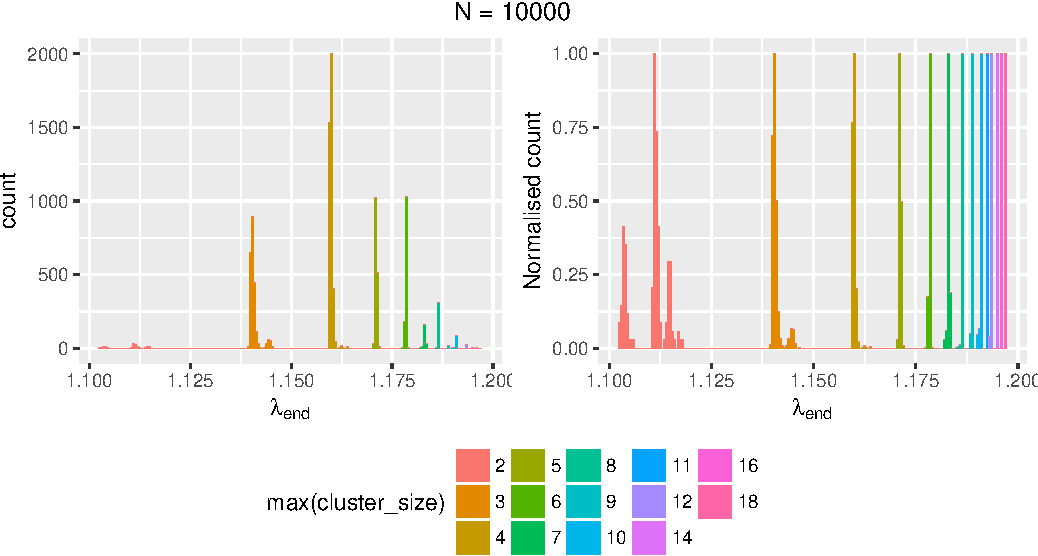
\includegraphics{index_files/figure-latex/vis__max_cluster-1.pdf}
\caption{\label{fig:vis__max_cluster} \(\lambda_{end}\) for randomly
sampled spatial configurations. Left: Plotted with raw count; Right:
Count is normalised for each \(max(cluster\_size)\) so that highest bar
measures 1.0}
\end{figure}

\begin{verbatim}
## Analysis of Variance Table
## 
## Response: lambda_end
##                           Df  Sum Sq Mean Sq F value    Pr(>F)    
## as.numeric(max_cluster)    1 1.89003 1.89003   41707 < 2.2e-16 ***
## Residuals               9998 0.45308 0.00005                      
## ---
## Signif. codes:  0 '***' 0.001 '**' 0.01 '*' 0.05 '.' 0.1 ' ' 1
\end{verbatim}

\subsubsection{Conclusion}\label{conclusion}

We have investigated the growth-dispersal model using
final-steady-growth-rate \(\lambda_{end}\) as a proxy, with the simple
case where \(\lambda(s)\) can only take two values, \(\lambda_{good}\)
or \(\lambda_{bad}\). Under such condition, we observe that
\(\lambda_{end}\) is dominated by the biggest cluster of good patches.
More generally, separation \(K=0\) and \(K=1\) are the most interesting
cases, where cluster interaction produces the complex outputs. Thus it
may be possible to model the \(\lambda_{end}\) by convolving
\(\lambda(s)\) with a local filter and then taking the maximum of the
resultant function. The exact form, however, is yet to be defined.

\section{References:}\label{references}

\hypertarget{refs}{}
\hypertarget{ref-Ellner2011}{}
{[}1{]} Ellner SP, Guckenheimer J. An introduction to R for dynamic
models in biology Department of Mathematics. 2011.

\section{Appendix:}\label{appendix}

\subsection{Figures}\label{figures}

\begin{figure}
\centering
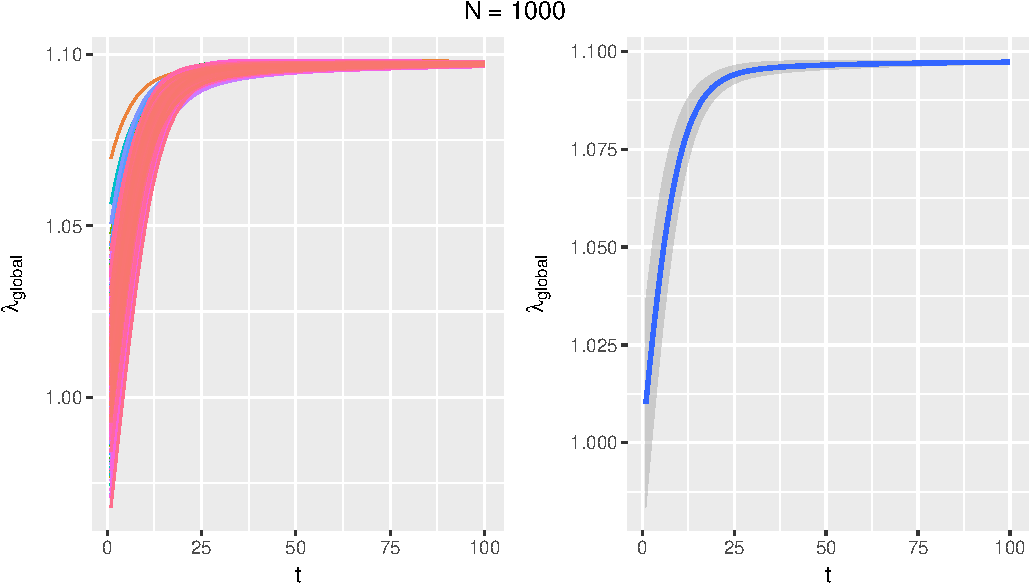
\includegraphics{index_files/figure-latex/vis__N1-1.pdf}
\caption{\label{fig:vis__N1} \(\lambda_{global}(t)\) for
\(N_1(s)\sim unif(0,100)\)}
\end{figure}

\subsection{R-scripts used:}\label{r-scripts-used}

\subsubsection{\texorpdfstring{``index.R'': the main script that
generates the
document}{index.R: the main script that generates the document}}\label{index.r-the-main-script-that-generates-the-document}

\begin{Shaded}
\begin{Highlighting}[]
\NormalTok{## ----word1, echo=F, inclue = T-------------------------------------------}

\NormalTok{#### Define utility function}
\StringTok{'%f%'}\NormalTok{ <-}\StringTok{ }\ControlFlowTok{function}\NormalTok{(x,f) \{ }\KeywordTok{do.call}\NormalTok{(}\DataTypeTok{what =}\NormalTok{ f,}
                                 \DataTypeTok{args =} \KeywordTok{list}\NormalTok{(x)) \}}

\NormalTok{#### Read data from file}
\NormalTok{f =}\StringTok{ }\KeywordTok{file}\NormalTok{(}\StringTok{'rpc2017/a1/usr-share-dict-words'}\NormalTok{,}\StringTok{'r'}\NormalTok{)}
\NormalTok{words  <-}\StringTok{  }\KeywordTok{readLines}\NormalTok{(f)}
\KeywordTok{close}\NormalTok{(f)}

\NormalTok{#### Convert to uppercase and count unique number}
\NormalTok{words <-}\StringTok{ }\KeywordTok{toupper}\NormalTok{(words)}
\NormalTok{words <-}\StringTok{ }\KeywordTok{unique}\NormalTok{(words)}
\KeywordTok{sprintf}\NormalTok{(}\StringTok{'A: %d'}\NormalTok{, }\KeywordTok{length}\NormalTok{(words))}\OperatorTok\NormalTok{cat;}

\NormalTok{## ----word2, echo=F-------------------------------------------------------}
\NormalTok{buf <-}\StringTok{ }\KeywordTok{c}\NormalTok{()}
\NormalTok{match_idx <-}\StringTok{ }\KeywordTok{grep}\NormalTok{(}\StringTok{'}\CharTok{\textbackslash{}'}\StringTok{'}\NormalTok{,words)}
\NormalTok{buf <-}\StringTok{ }\KeywordTok{c}\NormalTok{(buf,}\KeywordTok{sprintf}\NormalTok{(}\StringTok{'A: %d '}\NormalTok{, }\KeywordTok{length}\NormalTok{(match_idx)))}

\NormalTok{######### Print hits}
\NormalTok{hlen =}\StringTok{ }\DecValTok{10}
\NormalTok{df =}\StringTok{ }\KeywordTok{data.frame}\NormalTok{( words[match_idx])}
\NormalTok{caption =}\StringTok{ }\KeywordTok{sprintf}\NormalTok{(}\StringTok{'Showing best %d hits below:'}\NormalTok{,hlen)}
\NormalTok{knitr}\OperatorTok{::}\KeywordTok{kable}\NormalTok{( }
  \KeywordTok{head}\NormalTok{(df,hlen),}
  \DataTypeTok{booktabs =} \OtherTok{TRUE}\NormalTok{,}
  \DataTypeTok{caption =}\NormalTok{ caption}
\NormalTok{)}
\NormalTok{words <-}\StringTok{ }\NormalTok{words[}\OperatorTok{-}\NormalTok{match_idx]}
\NormalTok{buf <-}\StringTok{ }\KeywordTok{c}\NormalTok{(buf,}\KeywordTok{sprintf}\NormalTok{(}\StringTok{'}\CharTok{\textbackslash{}n}\StringTok{%d words left after filtering'}\NormalTok{, }\KeywordTok{length}\NormalTok{(words)))}
\NormalTok{buf}\OperatorTok\NormalTok{cat}

\NormalTok{## ----word3, echo=F-------------------------------------------------------}
\NormalTok{buf <-}\StringTok{ }\KeywordTok{c}\NormalTok{()}
\NormalTok{match_idx <-}\StringTok{ }\KeywordTok{grep}\NormalTok{(}\StringTok{'[^ -~]'}\NormalTok{,words)}
\NormalTok{buf <-}\StringTok{ }\KeywordTok{c}\NormalTok{(buf,}\KeywordTok{sprintf}\NormalTok{(}\StringTok{'A: %d '}\NormalTok{, }\KeywordTok{length}\NormalTok{(match_idx)))}

\NormalTok{######### Print hits}
\NormalTok{hlen =}\StringTok{ }\DecValTok{10}
\NormalTok{df =}\StringTok{ }\KeywordTok{data.frame}\NormalTok{( words[match_idx])}
\NormalTok{caption =}\StringTok{ }\KeywordTok{sprintf}\NormalTok{(}\StringTok{'Showing best %d hits below:'}\NormalTok{,hlen)}
\NormalTok{knitr}\OperatorTok{::}\KeywordTok{kable}\NormalTok{( }
  \KeywordTok{head}\NormalTok{(df,hlen),}
  \DataTypeTok{booktabs =} \OtherTok{TRUE}\NormalTok{,}
  \DataTypeTok{caption =}\NormalTok{ caption}
\NormalTok{)}



\NormalTok{words <-}\StringTok{ }\NormalTok{words[}\OperatorTok{-}\NormalTok{match_idx]}
\NormalTok{words_data <-}\StringTok{ }\NormalTok{words}
\NormalTok{buf <-}\StringTok{ }\KeywordTok{c}\NormalTok{(buf,}\KeywordTok{sprintf}\NormalTok{(}\StringTok{'}\CharTok{\textbackslash{}n}\StringTok{%d words left after filtering, saved to "words_data"'}\NormalTok{, }\KeywordTok{length}\NormalTok{(words)))}
\NormalTok{buf}\OperatorTok\NormalTok{cat}

\NormalTok{## ----word4, echo=F-------------------------------------------------------}
\NormalTok{words_data <-}\StringTok{ }\KeywordTok{sort}\NormalTok{(words_data)}
\NormalTok{putative <-}\StringTok{ }\NormalTok{words_data[}
  \KeywordTok{endsWith}\NormalTok{(words_data, }\StringTok{'OG'}\NormalTok{)}
\NormalTok{  ]}
\NormalTok{target <-}\StringTok{ }\KeywordTok{vapply}\NormalTok{( putative}
\NormalTok{                  , }\DataTypeTok{FUN =}\NormalTok{ \{}\ControlFlowTok{function}\NormalTok{ (x) }\KeywordTok{paste0}\NormalTok{(x,}\StringTok{'UE'}\NormalTok{)\}}
\NormalTok{                  ,}\DataTypeTok{FUN.VALUE=}\StringTok{'char'}
\NormalTok{                  ,}\DataTypeTok{USE.NAMES=}\NormalTok{T)}
\NormalTok{XOGUE <-}\StringTok{ }\NormalTok{words_data[}\KeywordTok{match}\NormalTok{(target,words_data)]}
\NormalTok{XOG   <-}\StringTok{ }\NormalTok{putative }
\NormalTok{result <-}\StringTok{ }\KeywordTok{data.frame}\NormalTok{(XOG,}
\NormalTok{                     XOGUE,}
                     \DataTypeTok{row.names =} \OtherTok{NULL}\NormalTok{) }
\KeywordTok{colnames}\NormalTok{(result)<-}\StringTok{ }\KeywordTok{c}\NormalTok{(}\StringTok{"XOG"}\NormalTok{,}\StringTok{"XOGUE"}\NormalTok{) }
\NormalTok{result <-}\StringTok{ }\NormalTok{result[}\KeywordTok{complete.cases}\NormalTok{(result),]}
\KeywordTok{rownames}\NormalTok{(result) <-}\StringTok{ }\DecValTok{1}\OperatorTok{:}\KeywordTok{nrow}\NormalTok{(result)}
\KeywordTok{sprintf}\NormalTok{(}\StringTok{'%d pairs of words were found to conform "XOG"->"XOGUE" projection'}\NormalTok{, }\KeywordTok{nrow}\NormalTok{(result))}\OperatorTok\NormalTok{cat}
\CommentTok{# print(result,  row.names = T)}

\NormalTok{######### Print hits}
\NormalTok{hlen =}\StringTok{ }\DecValTok{10}
\NormalTok{df =}\StringTok{ }\NormalTok{result}
\NormalTok{caption =}\StringTok{ }\KeywordTok{sprintf}\NormalTok{(}\StringTok{'Showing best %d hits below:'}\NormalTok{,hlen)}
\NormalTok{knitr}\OperatorTok{::}\KeywordTok{kable}\NormalTok{( }
  \KeywordTok{head}\NormalTok{(df,hlen),}
  \DataTypeTok{booktabs =} \OtherTok{TRUE}\NormalTok{,}
  \DataTypeTok{caption =}\NormalTok{ caption,}
  \DataTypeTok{align =} \StringTok{'l'}
\NormalTok{)}



\NormalTok{## ----word5,echo=F--------------------------------------------------------}
\NormalTok{fname =}\StringTok{ 'rpc2017/a1/scrabble.txt'}
\NormalTok{f =}\StringTok{ }\KeywordTok{file}\NormalTok{(fname,}\StringTok{'r'}\NormalTok{)}
\NormalTok{buf =}\StringTok{ }\NormalTok{f}\OperatorTok\NormalTok{readLines}
\NormalTok{buf =}\StringTok{ }\KeywordTok{strsplit}\NormalTok{(buf,}\StringTok{' '}\NormalTok{)}
\NormalTok{f}\OperatorTok\NormalTok{close}
\NormalTok{buf =}\StringTok{ }\KeywordTok{t}\NormalTok{(}\KeywordTok{array}\NormalTok{(}\KeywordTok{unlist}\NormalTok{(buf),}\DataTypeTok{dim =} \KeywordTok{c}\NormalTok{(}\KeywordTok{length}\NormalTok{(buf[[}\DecValTok{1}\NormalTok{]]),}\KeywordTok{length}\NormalTok{(buf) )))}
\NormalTok{buf <-}\StringTok{ }\NormalTok{buf[}\KeywordTok{order}\NormalTok{(buf[,}\DecValTok{1}\NormalTok{]),]}

\NormalTok{l =}\StringTok{ }\KeywordTok{length}\NormalTok{(}\KeywordTok{unique}\NormalTok{(buf[,}\DecValTok{1}\NormalTok{]))}
\ControlFlowTok{if}\NormalTok{ (l }\OperatorTok{!=}\StringTok{ }\DecValTok{26}\NormalTok{)\{}
\NormalTok{  msg =}\StringTok{ }\KeywordTok{paste0}\NormalTok{(}\StringTok{'[WARNING]: scrabble scores incomplete, expected 26, actual '}\NormalTok{,l)}
  \KeywordTok{warning}\NormalTok{(msg)}
\NormalTok{\}}
\CommentTok{# data.frame( char = buf[,1], score = buf[,4]) %f%print}
\NormalTok{scores <-}\StringTok{ }\NormalTok{buf[,}\KeywordTok{ncol}\NormalTok{(buf)] }\OperatorTok\StringTok{ }\NormalTok{as.integer}
\KeywordTok{names}\NormalTok{(scores) <-}\StringTok{ }\NormalTok{buf[,}\DecValTok{1}\NormalTok{]}
\NormalTok{hlen =}\StringTok{ }\DecValTok{10}
\NormalTok{df =}\StringTok{ }\KeywordTok{data.frame}\NormalTok{(}\DataTypeTok{scores =} \KeywordTok{sort}\NormalTok{(scores,}\DataTypeTok{decreasing =}\NormalTok{ T))}

\NormalTok{caption =}\StringTok{ }\KeywordTok{sprintf}\NormalTok{(}\StringTok{'Showing best %d hits below:'}\NormalTok{,hlen)}
\NormalTok{knitr}\OperatorTok{::}\KeywordTok{kable}\NormalTok{(}
  \KeywordTok{head}\NormalTok{(df,hlen),}
  \DataTypeTok{booktabs =} \OtherTok{TRUE}\NormalTok{,}
  \DataTypeTok{caption =}\NormalTok{ caption,}
  \DataTypeTok{align =} \StringTok{'l'}

\NormalTok{)}


\NormalTok{## ----word6,echo = F------------------------------------------------------}
\NormalTok{x =}\StringTok{ }\NormalTok{words_data}
\NormalTok{scoreit =}\StringTok{ }\NormalTok{\{}\ControlFlowTok{function}\NormalTok{ (x)\{}
                      \KeywordTok{sum}\NormalTok{(}
                          \KeywordTok{unlist}\NormalTok{(}
                            \KeywordTok{lapply}\NormalTok{( }\KeywordTok{strsplit}\NormalTok{(x,}\StringTok{''}\NormalTok{),}
                            \DataTypeTok{FUN =}\NormalTok{ \{}\ControlFlowTok{function}\NormalTok{(i) scores[i]\}}
\NormalTok{                            )}
\NormalTok{                          )}
\NormalTok{                      )}
\NormalTok{                    \}}
\NormalTok{          \}}
\NormalTok{y <-}\StringTok{ }\KeywordTok{sapply}\NormalTok{( x,}
                   \DataTypeTok{FUN =}\NormalTok{ scoreit,}
                  \CommentTok{# FUN.VALUE='integer',}
                  \DataTypeTok{USE.NAMES=}\NormalTok{T)}
\NormalTok{dy <-}\StringTok{ }\KeywordTok{density}\NormalTok{( y, }\DataTypeTok{bw =} \FloatTok{0.6}\NormalTok{)}
\CommentTok{# par(mar=c(3,3,3,3))}
\KeywordTok{plot}\NormalTok{( dy,}
      \DataTypeTok{main=}\StringTok{'Distribution of scrabble scores'}\NormalTok{)}
\NormalTok{my =}\StringTok{ }\KeywordTok{mean}\NormalTok{(y)}
\KeywordTok{abline}\NormalTok{( }\DataTypeTok{v =}\NormalTok{ my, }\DataTypeTok{col=}\DecValTok{2}\NormalTok{ )}
\KeywordTok{text}\NormalTok{(my, }\KeywordTok{median}\NormalTok{(dy}\OperatorTok{$}\NormalTok{y),}\KeywordTok{sprintf}\NormalTok{(}\StringTok{'mean=%.3f'}\NormalTok{,my), }\DataTypeTok{col =} \DecValTok{2}\NormalTok{)}

\NormalTok{#### DEBUG stats}
\ControlFlowTok{if}\NormalTok{ (debug)\{dy}\OperatorTok\NormalTok{print\}}

\KeywordTok{cat}\NormalTok{(}
  \StringTok{"Highest score is achieved by:"}\NormalTok{,}
  \KeywordTok{names}\NormalTok{(y)[idx<-}\KeywordTok{which.max}\NormalTok{(y)],}
  \StringTok{", Score:"}\NormalTok{,}
\NormalTok{  y[idx]}
\NormalTok{)}

\NormalTok{## ----word7---------------------------------------------------------------}
\NormalTok{##################################################################}
\NormalTok{#### compile reverse complement and define functions #############}
\NormalTok{##################################################################}
\NormalTok{dict =}\StringTok{ }\KeywordTok{rev}\NormalTok{(LETTERS)}
\KeywordTok{names}\NormalTok{(dict) <-}\StringTok{ }\NormalTok{LETTERS }

\NormalTok{rev_comp =}\StringTok{ }\ControlFlowTok{function}\NormalTok{(x)\{}
  \KeywordTok{paste0}\NormalTok{(}
    \KeywordTok{rev}\NormalTok{(dict[}\KeywordTok{unlist}\NormalTok{(}\KeywordTok{strsplit}\NormalTok{(x,}\StringTok{''}\NormalTok{))])}
\NormalTok{  ,}\DataTypeTok{collapse =} \StringTok{""}\NormalTok{)}
\NormalTok{\}}


\NormalTok{##################################################################}
\NormalTok{#### Carry out search }
\NormalTok{##################################################################}

\NormalTok{idx =}\StringTok{ }\KeywordTok{match}\NormalTok{(}
  \KeywordTok{sapply}\NormalTok{(words_data, }\DataTypeTok{FUN=}\NormalTok{rev_comp),}
\NormalTok{  words_data}
\NormalTok{)}\OperatorTok\NormalTok{na.omit}

\NormalTok{##################################################################}
\NormalTok{#### linking  WORDS to their reverse complements #################}
\NormalTok{#### Sort and format }
\NormalTok{##################################################################}
\NormalTok{rv_}\DecValTok{0}\NormalTok{ =}\StringTok{ }\NormalTok{words_data[idx]}
\NormalTok{rv_}\DecValTok{1}\NormalTok{ =}\StringTok{ }\KeywordTok{sapply}\NormalTok{( rv_}\DecValTok{0}\NormalTok{, }\DataTypeTok{FUN =}\NormalTok{ rev_comp )}

\NormalTok{res <-}\StringTok{ }\KeywordTok{data.frame}\NormalTok{(}
\NormalTok{  rv_}\DecValTok{0}\NormalTok{,}
\NormalTok{  rv_}\DecValTok{1}\NormalTok{)}
\NormalTok{res <-}\StringTok{  }\KeywordTok{apply}\NormalTok{(res, }\DataTypeTok{MARGIN =} \DecValTok{1}\NormalTok{, }\DataTypeTok{FUN =}\NormalTok{ sort)}\OperatorTok\NormalTok{t}
\NormalTok{dup_idx <-}\StringTok{ }\KeywordTok{duplicated}\NormalTok{(res[,}\DecValTok{1}\NormalTok{])}
\NormalTok{res <-}\StringTok{ }\NormalTok{res[}\OperatorTok{!}\NormalTok{dup_idx,]}
\NormalTok{res <-}\StringTok{ }\NormalTok{res[ }\KeywordTok{order}\NormalTok{(}\KeywordTok{nchar}\NormalTok{(res[,}\DecValTok{1}\NormalTok{]), }\DataTypeTok{decreasing =}\NormalTok{ T),]}

\KeywordTok{colnames}\NormalTok{(res) =}\StringTok{ }\KeywordTok{c}\NormalTok{(}\StringTok{'smaller_word'}\NormalTok{,}\StringTok{'larger_word'}\NormalTok{)}
\KeywordTok{rownames}\NormalTok{(res) <-}\StringTok{ }\DecValTok{1}\OperatorTok{:}\KeywordTok{nrow}\NormalTok{(res)}
\KeywordTok{sprintf}\NormalTok{(}\StringTok{'We found %d entries, out of which %d are reverse-complement to themselves , Showing longest 10 entries'}\NormalTok{, }\KeywordTok{nrow}\NormalTok{(res), }\KeywordTok{sum}\NormalTok{(res[,}\DecValTok{1}\NormalTok{]}\OperatorTok{==}\NormalTok{res[,}\DecValTok{2}\NormalTok{]),}\StringTok{'}\CharTok{\textbackslash{}n}\StringTok{'}\NormalTok{) }\OperatorTok\NormalTok{cat}

\NormalTok{######### Print hits}
\NormalTok{hlen =}\StringTok{ }\DecValTok{10}
\NormalTok{df =}\StringTok{ }\NormalTok{res}
\NormalTok{caption =}\StringTok{ }\KeywordTok{sprintf}\NormalTok{(}\StringTok{'Showing best %d hits below:'}\NormalTok{,hlen)}
\NormalTok{knitr}\OperatorTok{::}\KeywordTok{kable}\NormalTok{(}
  \KeywordTok{head}\NormalTok{(df,hlen),}
  \DataTypeTok{booktabs =} \OtherTok{TRUE}\NormalTok{,}
  \DataTypeTok{caption =}\NormalTok{ caption,}
  \DataTypeTok{align =} \StringTok{'l'}

\NormalTok{)}

\NormalTok{## ----word8---------------------------------------------------------------}
\NormalTok{count =}\StringTok{ }\ControlFlowTok{function}\NormalTok{(lst)\{}
  \KeywordTok{sapply}\NormalTok{(lst, \{}\ControlFlowTok{function}\NormalTok{(x)\{}
    \ControlFlowTok{if}\NormalTok{ (x[}\DecValTok{1}\NormalTok{]}\OperatorTok{==-}\DecValTok{1}\NormalTok{)\{}
      \DecValTok{0}
\NormalTok{    \}}\ControlFlowTok{else}\NormalTok{\{}
      \KeywordTok{length}\NormalTok{(x)}
\NormalTok{    \}}
\NormalTok{    \}\} )}
\NormalTok{\}}


\NormalTok{##### Define generic query function}
\NormalTok{search_perm <-}\StringTok{ }\ControlFlowTok{function}\NormalTok{ (}\DataTypeTok{query_orig_str =} \StringTok{'LLFAUYPNI'}\NormalTok{,}
                         \DataTypeTok{min_len =} \DecValTok{4}\NormalTok{,}
                        \DataTypeTok{database =}\NormalTok{  words_data,}
                        \DataTypeTok{special  =} \KeywordTok{c}\NormalTok{(}\StringTok{'A'}\NormalTok{)}
\NormalTok{                        )\{}
  
\NormalTok{  #### Preprocess the given string (vectorizing etc.)}
\NormalTok{  query_orig_str <-}\StringTok{ }\NormalTok{query_orig_str}
\NormalTok{  query_orig =}\StringTok{ }\KeywordTok{strsplit}\NormalTok{(query_orig_str,}\StringTok{''}\NormalTok{)[[}\DecValTok{1}\NormalTok{]]}

\NormalTok{  #### Obtain the unqiue set of chars}
\NormalTok{  query_uni =}\StringTok{ }\NormalTok{query_orig}\OperatorTok\NormalTok{unique}

\NormalTok{  #### Count occurrence of chars in the query}
\NormalTok{  qcount =}\StringTok{ }\KeywordTok{sapply}\NormalTok{( query_uni, }
\NormalTok{          \{}\ControlFlowTok{function}\NormalTok{(subq)}
\NormalTok{            \{}\KeywordTok{count}\NormalTok{(}
              \KeywordTok{gregexpr}\NormalTok{(subq, query_orig_str)}
\NormalTok{              )\}\})}
  
\NormalTok{  #### Counting occurence of chars for each word in database}
\NormalTok{  raw =}\StringTok{ }\KeywordTok{sapply}\NormalTok{( query_uni, }
\NormalTok{          \{}\ControlFlowTok{function}\NormalTok{(subq)}
\NormalTok{            \{}\KeywordTok{count}\NormalTok{(}
              \KeywordTok{gregexpr}\NormalTok{(subq, database)}
\NormalTok{              )\}\})}
  
  \ControlFlowTok{if}\NormalTok{(debug)\{}
\NormalTok{    raw0 <-}\StringTok{ }\NormalTok{raw}
\NormalTok{    raw <-}\StringTok{ }\NormalTok{raw0}
\NormalTok{  \}}
  
\NormalTok{  ### add index to initial dataset}
  \KeywordTok{rownames}\NormalTok{(raw) =}\StringTok{ }\DecValTok{1}\OperatorTok{:}\KeywordTok{nrow}\NormalTok{(raw)}
  
  
\NormalTok{  #### Exclude results that use more letters than specified}
\NormalTok{  exidx =}\StringTok{ }\KeywordTok{apply}\NormalTok{(}
    \KeywordTok{sweep}\NormalTok{(raw,qcount,}\DataTypeTok{MARGIN=}\DecValTok{2}\NormalTok{,}\DataTypeTok{FUN=}\NormalTok{\{}\ControlFlowTok{function}\NormalTok{(x,y) x}\OperatorTok{>}\NormalTok{y\}),}
    \DataTypeTok{MARGIN=}\DecValTok{1}\NormalTok{,}
    \DataTypeTok{FUN =}\NormalTok{ any )}
\NormalTok{  raw <-}\StringTok{ }\NormalTok{raw[}\OperatorTok{!}\NormalTok{exidx,]}
  
\NormalTok{  #### Exclude result that does not contain special chars}
\NormalTok{  exidx <-}\StringTok{ }\KeywordTok{apply}\NormalTok{(}
    \KeywordTok{sweep}\NormalTok{(raw}\OperatorTok{==}\DecValTok{0}\NormalTok{, query_uni }\OperatorTok\StringTok{ }\NormalTok{special,}
         \DataTypeTok{MARGIN =} \DecValTok{2}\NormalTok{,}
         \DataTypeTok{FUN =} \StringTok{'&'}\NormalTok{),}
        \DataTypeTok{MARGIN =} \DecValTok{1}\NormalTok{,}
        \DataTypeTok{FUN =}\NormalTok{ any)}
\NormalTok{  raw <-}\StringTok{ }\NormalTok{raw[}\OperatorTok{!}\NormalTok{exidx,]}
  
\NormalTok{  ###### Compile into a data.frame}
\NormalTok{  words_res =}\StringTok{ }\NormalTok{database[}\KeywordTok{rownames}\NormalTok{(raw)}\OperatorTok\NormalTok{as.integer]}
\NormalTok{  words_score =}\StringTok{ }\KeywordTok{apply}\NormalTok{( raw,}\DataTypeTok{MARGIN =} \DecValTok{1}\NormalTok{, sum)}
  
\NormalTok{  output =}\StringTok{ }\KeywordTok{data.frame}\NormalTok{(}
\NormalTok{    words_res,}
    \DataTypeTok{words_len =} \KeywordTok{nchar}\NormalTok{(words_res),}
\NormalTok{    words_score}
\NormalTok{    )}
  
\NormalTok{  ##################################################################}
\NormalTok{  #### Filtering out words that require additional characters ##############}
  
\NormalTok{  #### Option 1: Do not allow extra chars}
\NormalTok{  inidx <-}\StringTok{  }\NormalTok{output}\OperatorTok{$}\NormalTok{words_len}\OperatorTok{==}\NormalTok{output}\OperatorTok{$}\NormalTok{words_score }\OperatorTok{&}\StringTok{ }\NormalTok{output}\OperatorTok{$}\NormalTok{words_score}\OperatorTok{>=}\NormalTok{min_len}
  
\NormalTok{  #### Option 2: Do allow extra chars}
  \CommentTok{# inidx <-  output$words_score>=min_len}
  
\NormalTok{  output <-}\StringTok{ }\NormalTok{output[inidx,]}
  
\NormalTok{  odx =}\StringTok{ }\KeywordTok{order}\NormalTok{(output}\OperatorTok{$}\NormalTok{words_score,}\DataTypeTok{decreasing =}\NormalTok{ T)}
\NormalTok{  output <-}\StringTok{ }\NormalTok{output[odx,]}
\NormalTok{\}}


\NormalTok{### Actual evaluating the demanded query}
\NormalTok{query_orig_str =}\StringTok{ 'LLFAUYPNI'}
\NormalTok{min_len =}\StringTok{ }\DecValTok{4}
\NormalTok{database =}\StringTok{  }\NormalTok{words_data}
\NormalTok{special =}\StringTok{ }\KeywordTok{c}\NormalTok{(}\StringTok{'A'}\NormalTok{)}

\NormalTok{output <-}\StringTok{ }\KeywordTok{search_perm}\NormalTok{(}
    \DataTypeTok{query_orig_str =}\NormalTok{ query_orig_str,}
    \DataTypeTok{min_len =}\NormalTok{ min_len,}
    \DataTypeTok{database =}\NormalTok{  database,}
    \DataTypeTok{special =}\NormalTok{ special}
\NormalTok{)}

\NormalTok{#### Check correctness}
\ControlFlowTok{if}\NormalTok{ (}\KeywordTok{nrow}\NormalTok{(output) }\OperatorTok{!=}\StringTok{ }\DecValTok{39}\NormalTok{)}
\NormalTok{\{}
  \KeywordTok{warning}\NormalTok{(}\StringTok{"[WARNING]:Number of result is different from the cached one"}\NormalTok{)}
\NormalTok{\}}


\KeywordTok{sprintf}\NormalTok{(}\StringTok{'We found %d hits according to query }\CharTok{\textbackslash{}"}\StringTok{%s}\CharTok{\textbackslash{}"}\StringTok{ in }\CharTok{\textbackslash{}"}\StringTok{words_data}\CharTok{\textbackslash{}"}\StringTok{", }\CharTok{\textbackslash{}n}\StringTok{ (Option: min_len=%d, special=%s). '}\NormalTok{, }\KeywordTok{nrow}\NormalTok{(output), query_orig_str, min_len ,}\KeywordTok{paste0}\NormalTok{(special,}\DataTypeTok{collapse =} \StringTok{','}\NormalTok{))}\OperatorTok\NormalTok{cat}
\CommentTok{# sprintf('Showing best %d hits below:',hlen) %f% cat}

\NormalTok{######### Print hits}
\NormalTok{hlen =}\StringTok{ }\DecValTok{20}
\NormalTok{df =}\StringTok{ }\NormalTok{output}
\NormalTok{caption =}\StringTok{ }\KeywordTok{sprintf}\NormalTok{(}\StringTok{'Showing best %d hits below:'}\NormalTok{,hlen)}
\NormalTok{knitr}\OperatorTok{::}\KeywordTok{kable}\NormalTok{(}
  \KeywordTok{head}\NormalTok{(df,hlen),}
  \DataTypeTok{booktabs =} \OtherTok{TRUE}\NormalTok{,}
  \DataTypeTok{caption =}\NormalTok{ caption,}
  \DataTypeTok{align =} \StringTok{'l'}
\NormalTok{)}


\NormalTok{## ----exam1---------------------------------------------------------------}
\NormalTok{#### Read data }
\KeywordTok{setwd}\NormalTok{(}\StringTok{'rpc2017/a1/grading/'}\NormalTok{)}


\NormalTok{##### read correct answers into "ref"}
\NormalTok{fname =}\StringTok{ "crib.dat"}
\NormalTok{f =}\StringTok{ }\KeywordTok{file}\NormalTok{( fname,}\StringTok{'r'}\NormalTok{)}
\NormalTok{ref  <-}\StringTok{  }\KeywordTok{readLines}\NormalTok{(f)}
\KeywordTok{close}\NormalTok{(f)}
\NormalTok{qnum <-}\StringTok{ }\KeywordTok{length}\NormalTok{(ref)}
\NormalTok{qlevel =}\StringTok{ }\KeywordTok{unique}\NormalTok{(ref)}\OperatorTok\NormalTok{sort}
\NormalTok{qdict <-}\StringTok{ }\DecValTok{1}\OperatorTok{:}\KeywordTok{length}\NormalTok{(qlevel)}
\KeywordTok{names}\NormalTok{(qdict) <-}\StringTok{ }\NormalTok{qlevel}

\KeywordTok{sprintf}\NormalTok{(}\StringTok{"[DEBUG]:There are %d questions from file:%s"}\NormalTok{,qnum,fname)}\OperatorTok\NormalTok{cat}

\NormalTok{####### Loading grading scheme and transform it to a vector}
\NormalTok{grade_crit <-}\StringTok{ }\KeywordTok{read.table}\NormalTok{(}\DataTypeTok{file =} \StringTok{'grade.txt'}\NormalTok{,}\DataTypeTok{header =}\NormalTok{ T)}
\NormalTok{grade_dict <-}\StringTok{ }\KeywordTok{rep}\NormalTok{(}\DecValTok{0}\NormalTok{,}\DecValTok{101}\NormalTok{)}
\ControlFlowTok{for}\NormalTok{ (i }\ControlFlowTok{in} \DecValTok{1}\OperatorTok{:}\KeywordTok{nrow}\NormalTok{(grade_crit))\{}
\NormalTok{  ROW <-}\StringTok{ }\NormalTok{grade_crit[i,]}
\NormalTok{  MIN =}\StringTok{ }\NormalTok{ROW[[}\DecValTok{1}\NormalTok{]]}
\NormalTok{  MAX =}\StringTok{ }\NormalTok{ROW[[}\DecValTok{2}\NormalTok{]]}
\NormalTok{  grade =}\StringTok{ }\NormalTok{ROW[[}\DecValTok{3}\NormalTok{]]}
\NormalTok{  grade_dict[ MIN}\OperatorTok{:}\NormalTok{MAX }\OperatorTok{+}\StringTok{ }\DecValTok{1}\NormalTok{] <-}\StringTok{ }\NormalTok{grade  }
\NormalTok{\}}
\NormalTok{grade_dict <-}\StringTok{ }\KeywordTok{factor}\NormalTok{(grade_dict, }\DataTypeTok{labels =}\NormalTok{ grade_crit}\OperatorTok{$}\NormalTok{grade}\OperatorTok\NormalTok{levels) }
\NormalTok{graduate <-}\StringTok{ }\ControlFlowTok{function}\NormalTok{(x)\{grade_dict[x}\OperatorTok{+}\DecValTok{1}\NormalTok{]\}}

\NormalTok{##### Test }
\ControlFlowTok{if}\NormalTok{ ( }\KeywordTok{any}\NormalTok{(}\OperatorTok{!}\KeywordTok{graduate}\NormalTok{(}\KeywordTok{c}\NormalTok{(}\DecValTok{39}\NormalTok{,}\DecValTok{40}\NormalTok{,}\DecValTok{49}\NormalTok{,}\DecValTok{50}\NormalTok{,}\DecValTok{59}\NormalTok{,}\DecValTok{60}\NormalTok{,}\DecValTok{69}\NormalTok{,}\DecValTok{70}\NormalTok{)) }\OperatorTok{==}\StringTok{ }\KeywordTok{c}\NormalTok{(}\StringTok{'F'}\NormalTok{,}\StringTok{'D'}\NormalTok{,}\StringTok{'D'}\NormalTok{,}\StringTok{'C'}\NormalTok{,}\StringTok{'C'}\NormalTok{,}\StringTok{'B'}\NormalTok{,}\StringTok{'B'}\NormalTok{,}\StringTok{'A'}\NormalTok{)) )\{}
  \KeywordTok{warning}\NormalTok{(}\StringTok{"[WARNING]:Cannot safely define }\CharTok{\textbackslash{}"}\StringTok{graduate()}\CharTok{\textbackslash{}"}\StringTok{"}\NormalTok{)}
\NormalTok{\}}

\NormalTok{##### Read results for each student}
\NormalTok{buf =}\StringTok{ }\KeywordTok{list}\NormalTok{()}
\NormalTok{resp =}\StringTok{ }\KeywordTok{list}\NormalTok{()}
\ControlFlowTok{for}\NormalTok{ (fname }\ControlFlowTok{in} \KeywordTok{list.files}\NormalTok{(}\KeywordTok{getwd}\NormalTok{()))\{}
  \ControlFlowTok{if}\NormalTok{ ( }\KeywordTok{startsWith}\NormalTok{(fname,}\StringTok{'student'}\NormalTok{) )\{}
    
\NormalTok{  ##### Extract student number from filename and read data}
\NormalTok{  idx =}\StringTok{ }\KeywordTok{regmatches}\NormalTok{( fname,}\KeywordTok{gregexpr}\NormalTok{(}\StringTok{"[0-9]+"}\NormalTok{, fname))}\OperatorTok\NormalTok{as.integer}
\NormalTok{  f =}\StringTok{ }\KeywordTok{file}\NormalTok{(fname,}\StringTok{'r'}\NormalTok{)}
\NormalTok{  ttbl <-}\StringTok{ }\KeywordTok{read.table}\NormalTok{(f, }\DataTypeTok{header =}\NormalTok{ T,}\DataTypeTok{stringsAsFactors =}\NormalTok{ F)}
  \KeywordTok{close}\NormalTok{(f)}
\NormalTok{  ##### score answers and cache answers to "resp"}
\NormalTok{  score =}\StringTok{ }\KeywordTok{sum}\NormalTok{(ref[ttbl}\OperatorTok{$}\NormalTok{qn] }\OperatorTok{==}\StringTok{ }\NormalTok{ttbl}\OperatorTok{$}\NormalTok{response)}
\NormalTok{  buf[[idx]] =}\StringTok{ }\KeywordTok{list}\NormalTok{( }\DataTypeTok{student_idx =}\NormalTok{ idx, }
                     \DataTypeTok{score =}\NormalTok{ score, }
                     \DataTypeTok{qnum =} \KeywordTok{nrow}\NormalTok{(ttbl)}
\NormalTok{                     )}
\NormalTok{  ttbl}\OperatorTok{$}\NormalTok{response <-}\StringTok{ }\NormalTok{qdict[ttbl}\OperatorTok{$}\NormalTok{response] }
\NormalTok{  resp[[idx]] =}\StringTok{ }\NormalTok{ttbl}
\NormalTok{  \}}
\NormalTok{\}}

\NormalTok{#### Compile data frame}
\NormalTok{df <-}\StringTok{ }\KeywordTok{data.frame}\NormalTok{(}\KeywordTok{matrix}\NormalTok{(}\KeywordTok{unlist}\NormalTok{(buf), }\DataTypeTok{nrow=}\KeywordTok{length}\NormalTok{(buf), }\DataTypeTok{byrow=}\NormalTok{T))}
\KeywordTok{colnames}\NormalTok{(df) <-}\StringTok{ }\KeywordTok{names}\NormalTok{(buf[[}\DecValTok{1}\NormalTok{]])}
\NormalTok{df}\OperatorTok{$}\NormalTok{percent <-}\StringTok{ }\KeywordTok{floor}\NormalTok{(df}\OperatorTok{$}\NormalTok{score }\OperatorTok{/}\StringTok{ }\NormalTok{df}\OperatorTok{$}\NormalTok{qnum }\OperatorTok{*}\StringTok{ }\DecValTok{100}\NormalTok{)}
\NormalTok{df}\OperatorTok{$}\NormalTok{grade <-}\StringTok{ }\NormalTok{df}\OperatorTok{$}\NormalTok{percent}\OperatorTok\NormalTok{graduate}
\NormalTok{df}\OperatorTok{$}\NormalTok{rank <-}\StringTok{ }\KeywordTok{rank}\NormalTok{(}\OperatorTok{-}\NormalTok{df}\OperatorTok{$}\NormalTok{percent)}
\NormalTok{df <-}\StringTok{ }\NormalTok{df[}\KeywordTok{order}\NormalTok{(}\OperatorTok{-}\NormalTok{df}\OperatorTok{$}\NormalTok{score),]}
\ControlFlowTok{if}\NormalTok{ (}\KeywordTok{sd}\NormalTok{(df}\OperatorTok{$}\NormalTok{qnum)}\OperatorTok{!=}\DecValTok{0}\NormalTok{)\{}
  \KeywordTok{warning}\NormalTok{(}\StringTok{"Question answered is not homogeneous"}\NormalTok{)}
\NormalTok{\}}

\NormalTok{df <-}\StringTok{ }\KeywordTok{subset}\NormalTok{(df,}\DataTypeTok{select =} \OperatorTok{-}\KeywordTok{c}\NormalTok{(qnum)) #### Drop columns for better printout}
\NormalTok{hlen <-}\StringTok{ }\KeywordTok{nrow}\NormalTok{(df)}
\NormalTok{caption =}\StringTok{ }\KeywordTok{sprintf}\NormalTok{(}\StringTok{'Result of %d students in this exam, sorted by percent score in descending order'}\NormalTok{, }\KeywordTok{nrow}\NormalTok{(df) )}
\NormalTok{knitr}\OperatorTok{::}\KeywordTok{kable}\NormalTok{( }
  \KeywordTok{head}\NormalTok{(df,hlen),}
  \DataTypeTok{booktabs =} \OtherTok{TRUE}\NormalTok{,}
  \DataTypeTok{caption =}\NormalTok{ caption,}
  \DataTypeTok{row.names =}\NormalTok{ F}
  \CommentTok{# align = 'l'}
\NormalTok{)}
\KeywordTok{sprintf}\NormalTok{(}\StringTok{"Stats were calculated for the rounded percent score for %d students in the exam"}\NormalTok{, }\KeywordTok{nrow}\NormalTok{(df))}\OperatorTok\NormalTok{cat}
\KeywordTok{summary}\NormalTok{(df}\OperatorTok{$}\NormalTok{percent)}\OperatorTok\NormalTok{print}
\NormalTok{res_exam <-}\StringTok{ }\NormalTok{df}


\NormalTok{## ----exam_naive,fig.cap=" \textbackslash{}\textbackslash{}label\{fig:exam_naive\} Distribution of $I_\{cheat\}$"----}
\NormalTok{idx_xy <-}\StringTok{ }\KeywordTok{t}\NormalTok{(}\KeywordTok{combn}\NormalTok{(}\DecValTok{1}\OperatorTok{:}\KeywordTok{nrow}\NormalTok{(res_exam),}\DecValTok{2}\NormalTok{))}
\NormalTok{res_exam <-}\StringTok{ }\NormalTok{res_exam[}\KeywordTok{order}\NormalTok{(res_exam}\OperatorTok{$}\NormalTok{student_idx),]}

\CommentTok{# df <- res_exam}
\NormalTok{cindex <-}\StringTok{ }\ControlFlowTok{function}\NormalTok{(sa,sb,}\DataTypeTok{df =}\NormalTok{ resp)\{}
\NormalTok{  sumA <-}\StringTok{ }\KeywordTok{intersect}\NormalTok{(df[[sa]]}\OperatorTok{$}\NormalTok{qn,df[[sb]]}\OperatorTok{$}\NormalTok{qn) }\OperatorTok\StringTok{ }\NormalTok{length}
\NormalTok{  sumB <-}\StringTok{ }\KeywordTok{intersect}\NormalTok{(}\KeywordTok{data.frame}\NormalTok{(}\KeywordTok{t}\NormalTok{(df[[sa]]))}
\NormalTok{            ,}\KeywordTok{data.frame}\NormalTok{(}\KeywordTok{t}\NormalTok{(df[[sb]]))}
\NormalTok{              )}\OperatorTok\StringTok{ }\NormalTok{ncol}
  \KeywordTok{c}\NormalTok{(sumA,sumB)}
\NormalTok{  \}  }

\NormalTok{overlap <-}\StringTok{ }\KeywordTok{apply}\NormalTok{(idx_xy, }\DataTypeTok{MARGIN =} \DecValTok{1}\NormalTok{, }\DataTypeTok{FUN =}\NormalTok{ \{}\ControlFlowTok{function}\NormalTok{(x) }
  \KeywordTok{cindex}\NormalTok{( x[}\DecValTok{1}\NormalTok{],x[}\DecValTok{2}\NormalTok{])}
\NormalTok{\}}
\NormalTok{)}\OperatorTok\NormalTok{t}
\NormalTok{I_cheat <-}\StringTok{ }\NormalTok{overlap[,}\DecValTok{2}\NormalTok{]}\OperatorTok{/}\NormalTok{overlap[,}\DecValTok{1}\NormalTok{]}
\KeywordTok{hist}\NormalTok{(I_cheat,}\DataTypeTok{main =} \OtherTok{NULL}\NormalTok{);}


\NormalTok{## ----exam_diag, fig.cap= cap---------------------------------------------}

\NormalTok{cap <-}\StringTok{ "}\CharTok{\textbackslash{}\textbackslash{}}\StringTok{label\{fig:exam_diag\} Diagnostic plots for finding the outlier/cheater"}

\NormalTok{##### Calculate naive cheat index}
\NormalTok{idx_xy <-}\StringTok{ }\KeywordTok{t}\NormalTok{(}\KeywordTok{combn}\NormalTok{(}\DecValTok{1}\OperatorTok{:}\KeywordTok{nrow}\NormalTok{(res_exam),}\DecValTok{2}\NormalTok{))}
\NormalTok{res_exam <-}\StringTok{ }\NormalTok{res_exam[}\KeywordTok{order}\NormalTok{(res_exam}\OperatorTok{$}\NormalTok{student_idx),]}

\NormalTok{cindex <-}\StringTok{ }\ControlFlowTok{function}\NormalTok{(sa,sb,}\DataTypeTok{df =}\NormalTok{ resp)\{}
\NormalTok{  sumA <-}\StringTok{ }\KeywordTok{intersect}\NormalTok{(df[[sa]]}\OperatorTok{$}\NormalTok{qn,df[[sb]]}\OperatorTok{$}\NormalTok{qn) }\OperatorTok\StringTok{ }\NormalTok{length}
\NormalTok{  sumB <-}\StringTok{ }\KeywordTok{intersect}\NormalTok{(}\KeywordTok{data.frame}\NormalTok{(}\KeywordTok{t}\NormalTok{(df[[sa]]))}
\NormalTok{            ,}\KeywordTok{data.frame}\NormalTok{(}\KeywordTok{t}\NormalTok{(df[[sb]]))}
\NormalTok{              )}\OperatorTok\StringTok{ }\NormalTok{ncol}
  \KeywordTok{c}\NormalTok{(sumA,sumB)}
\NormalTok{  \}  }


\NormalTok{#### take two students and find overlap in choic of questions}
\NormalTok{overlap <-}\StringTok{ }\KeywordTok{apply}\NormalTok{(idx_xy, }\DataTypeTok{MARGIN =} \DecValTok{1}\NormalTok{, }\DataTypeTok{FUN =}\NormalTok{ \{}\ControlFlowTok{function}\NormalTok{(x) }
  \KeywordTok{cindex}\NormalTok{( x[}\DecValTok{1}\NormalTok{],x[}\DecValTok{2}\NormalTok{])}
\NormalTok{\}}
\NormalTok{)}\OperatorTok\NormalTok{t}
\NormalTok{question_overlap <-}\StringTok{ }\NormalTok{overlap[,}\DecValTok{1}\NormalTok{]}
\NormalTok{answer_overlap <-}\StringTok{ }\NormalTok{overlap[,}\DecValTok{2}\NormalTok{]}
\NormalTok{x <-}\StringTok{ }\NormalTok{question_overlap}
\NormalTok{y <-}\StringTok{ }\NormalTok{answer_overlap}

\NormalTok{#### regression}
\NormalTok{mdl <-}\StringTok{ }\KeywordTok{lm}\NormalTok{(y}\OperatorTok{~}\NormalTok{x)}
\NormalTok{mdl}\OperatorTok{$}\NormalTok{stdres <-}\StringTok{ }\KeywordTok{rstandard}\NormalTok{(mdl)}

\NormalTok{###### Thresholding outliers}
\NormalTok{conf <-}\StringTok{  }\FloatTok{0.975}\NormalTok{ #### 1-tail p-value}
\NormalTok{cap <-}\StringTok{ }\KeywordTok{paste0}\NormalTok{(cap,}
\KeywordTok{sprintf}\NormalTok{(}\StringTok{"}\CharTok{\textbackslash{}\textbackslash{}}\StringTok{newline (Using %.3f %% confidence (2 tailed) as threshold)"}\NormalTok{, (}\DecValTok{2} \OperatorTok{*}\StringTok{ }\NormalTok{conf }\OperatorTok{-}\StringTok{ }\DecValTok{1}\NormalTok{ )}\OperatorTok{*}\DecValTok{100}\NormalTok{)}
\NormalTok{              )}
\NormalTok{zlim <-}\StringTok{ }\KeywordTok{qnorm}\NormalTok{(conf)}
\NormalTok{outliers <-}\StringTok{ }\KeywordTok{which}\NormalTok{( }\KeywordTok{abs}\NormalTok{(mdl}\OperatorTok{$}\NormalTok{stdres) }\OperatorTok{>}\StringTok{ }\NormalTok{zlim)}

\NormalTok{##### Print plots}
\KeywordTok{par}\NormalTok{(}\DataTypeTok{mfrow=}\KeywordTok{c}\NormalTok{(}\DecValTok{1}\NormalTok{,}\DecValTok{2}\NormalTok{))}
\KeywordTok{plot}\NormalTok{(x,y,}
     \DataTypeTok{xlab =} \StringTok{"Number of overlapped questions"}\NormalTok{,}
     \DataTypeTok{ylab =} \StringTok{"Number of overlapped answers"}\NormalTok{,}
     \DataTypeTok{xlim =} \KeywordTok{c}\NormalTok{(}\OperatorTok{-}\DecValTok{1}\NormalTok{,}\DecValTok{35}\NormalTok{),}
     \DataTypeTok{ylim =} \KeywordTok{c}\NormalTok{(}\OperatorTok{-}\DecValTok{1}\NormalTok{,}\DecValTok{35}\NormalTok{)}
\NormalTok{    )}

\KeywordTok{text}\NormalTok{( x[outliers], y[outliers], outliers,}\DataTypeTok{adj =} \KeywordTok{c}\NormalTok{(}\OperatorTok{-}\NormalTok{.}\DecValTok{3}\NormalTok{,}\OperatorTok{-}\NormalTok{.}\DecValTok{3}\NormalTok{))}
\KeywordTok{abline}\NormalTok{(mdl,}\DataTypeTok{col =} \DecValTok{2}\NormalTok{)}

\KeywordTok{plot}\NormalTok{(mdl}\OperatorTok{$}\NormalTok{stdres,}\DataTypeTok{ylab=}\StringTok{'standardised residual'}\NormalTok{,}
     \DataTypeTok{ylim =} \KeywordTok{c}\NormalTok{(}\OperatorTok{-}\DecValTok{6}\NormalTok{,}\DecValTok{6}\NormalTok{))}
\KeywordTok{abline}\NormalTok{(}\DataTypeTok{h =}\NormalTok{ zlim, }\DataTypeTok{col=}\DecValTok{2}\NormalTok{)}
\KeywordTok{abline}\NormalTok{(}\DataTypeTok{h =}\OperatorTok{-}\NormalTok{zlim, }\DataTypeTok{col=}\DecValTok{2}\NormalTok{)}
\KeywordTok{abline}\NormalTok{(}\DataTypeTok{h =} \DecValTok{0}\NormalTok{,}\DataTypeTok{lty=}\DecValTok{2}\NormalTok{)}
\KeywordTok{text}\NormalTok{( outliers, mdl}\OperatorTok{$}\NormalTok{stdres[outliers], outliers,}\DataTypeTok{adj =} \KeywordTok{c}\NormalTok{(}\OperatorTok{-}\NormalTok{.}\DecValTok{3}\NormalTok{,}\OperatorTok{-}\NormalTok{.}\DecValTok{3}\NormalTok{))}

\NormalTok{#### compile data frame}
\NormalTok{cheats<-}\KeywordTok{data.frame}\NormalTok{(}
  \DataTypeTok{stud_A =}\NormalTok{ idx_xy[,}\DecValTok{1}\NormalTok{],}
  \DataTypeTok{grad   =}\NormalTok{ df}\OperatorTok{$}\NormalTok{grade[idx_xy[,}\DecValTok{1}\NormalTok{]],}
  \DataTypeTok{stud_B =}\NormalTok{ idx_xy[,}\DecValTok{2}\NormalTok{],}
  \DataTypeTok{grad   =}\NormalTok{ df}\OperatorTok{$}\NormalTok{grade[idx_xy[,}\DecValTok{2}\NormalTok{]],}
  \DataTypeTok{ques_same =}\NormalTok{ question_overlap,}
  \DataTypeTok{ans_same =}\NormalTok{ answer_overlap,}
  \DataTypeTok{zscore =}\NormalTok{ mdl}\OperatorTok{$}\NormalTok{stdres,}
  \DataTypeTok{Confidence_to_reject_NULL =} \DecValTok{2} \OperatorTok{*}\StringTok{ }\KeywordTok{pnorm}\NormalTok{(}\KeywordTok{abs}\NormalTok{(mdl}\OperatorTok{$}\NormalTok{stdres)) }\OperatorTok{-}\StringTok{ }\DecValTok{1}
\NormalTok{)}

\NormalTok{cheats <-}\StringTok{ }\NormalTok{cheats[}\KeywordTok{order}\NormalTok{(}\OperatorTok{-}\NormalTok{(cheats}\OperatorTok{$}\NormalTok{zscore)),]  }

\NormalTok{######### Print hits}
\NormalTok{hlen =}\StringTok{ }\DecValTok{10}
\NormalTok{df <-}\StringTok{ }\NormalTok{cheats}
\NormalTok{df <-}\StringTok{ }\KeywordTok{subset}\NormalTok{(df,}\DataTypeTok{select =} \OperatorTok{-}\KeywordTok{c}\NormalTok{(zscore)) #### Drop columns for better printout}
\NormalTok{caption =}\StringTok{ }\KeywordTok{sprintf}\NormalTok{(}\StringTok{'Showing best %d hits below:'}\NormalTok{,hlen)}
\NormalTok{knitr}\OperatorTok{::}\KeywordTok{kable}\NormalTok{(}
  \KeywordTok{head}\NormalTok{(df,hlen),}
  \DataTypeTok{booktabs =} \OtherTok{TRUE}\NormalTok{,}
  \DataTypeTok{caption =} \KeywordTok{paste0}\NormalTok{(}\StringTok{'}\CharTok{\textbackslash{}\textbackslash{}}\StringTok{label\{tab:exam_diag\}'}\NormalTok{,caption)}
\NormalTok{)}



\NormalTok{## ----DMB_log, fig.cap= cap,eval=T----------------------------------------}
\KeywordTok{source}\NormalTok{(}\StringTok{'DMB.R'}\NormalTok{)}
\NormalTok{#################################################}
\NormalTok{### simple visulisation of N(s,t) ###############}
\NormalTok{#################################################}
\NormalTok{cap <-}\StringTok{ " }\CharTok{\textbackslash{}\textbackslash{}}\StringTok{label\{fig:DMB_log\} Simple visualisation without taking differential "} 
\NormalTok{L=}\DecValTok{20}
\NormalTok{pop =}\StringTok{ }\KeywordTok{rep}\NormalTok{(}\DecValTok{5}\NormalTok{,L)}
\CommentTok{# pop <- rnorm(L,mean = 1, sd = 4 )}
\NormalTok{d<-}\StringTok{ }\FloatTok{0.1}
\NormalTok{rate <-}\StringTok{ }\KeywordTok{rep}\NormalTok{( }\KeywordTok{c}\NormalTok{(}\FloatTok{0.9}\NormalTok{,}\FloatTok{1.1}\NormalTok{),}\KeywordTok{c}\NormalTok{( L}\OperatorTok{/}\DecValTok{2}\NormalTok{, L}\OperatorTok{/}\DecValTok{2}\NormalTok{)) }\CommentTok{# %f% shuffle}
\CommentTok{# rate <- rep( c(0.9,1.1),c( L/2, L/2)) %f% shuffle}

\NormalTok{s0 <-}\StringTok{ }\KeywordTok{list}\NormalTok{(    }\DataTypeTok{pop =} \KeywordTok{pmax}\NormalTok{(}\DecValTok{0}\NormalTok{,pop),}
               \DataTypeTok{rate =} \KeywordTok{pmax}\NormalTok{(}\DecValTok{0}\NormalTok{,rate),}
               \DataTypeTok{filter=} \KeywordTok{c}\NormalTok{(d, }\DecValTok{1}\OperatorTok{-}\DecValTok{2}\OperatorTok{*}\NormalTok{d, d),}
               \DataTypeTok{nhis =} \DecValTok{500}
\NormalTok{               )}
\NormalTok{s0}\OperatorTok{$}\NormalTok{his <-}\StringTok{ }\KeywordTok{do.call}\NormalTok{(rbind, }\KeywordTok{rep}\NormalTok{(}\KeywordTok{list}\NormalTok{(pop), s0}\OperatorTok{$}\NormalTok{nhis))}
\NormalTok{s0}\OperatorTok{$}\NormalTok{L <-}\StringTok{ }\KeywordTok{length}\NormalTok{(s0}\OperatorTok{$}\NormalTok{pop)}
\NormalTok{s1<-s0}
\NormalTok{s1 <-}\StringTok{ }\KeywordTok{kickoff}\NormalTok{(s1,}\DecValTok{100}\NormalTok{)}
\CommentTok{# f <- function(x)\{log10(1+10*x)\}}
\KeywordTok{simple_vis}\NormalTok{(s1)}

\NormalTok{## ----DMB_logdiff,fig.cap = cap,eval = T----------------------------------}
\NormalTok{###################################################################}
\NormalTok{### visulisation of N(s,t) after taking differential w.r.t. time }
\NormalTok{###################################################################}
\NormalTok{cap <-}\StringTok{ " }\CharTok{\textbackslash{}\textbackslash{}}\StringTok{label\{fig:DMB_logdiff\} Visualisation after taking differential w.r.t. time"} 
\NormalTok{s1<-s0}
\NormalTok{s1 <-}\StringTok{ }\KeywordTok{kickoff}\NormalTok{(s1,}\DecValTok{500}\NormalTok{)}
\KeywordTok{diff_vis}\NormalTok{(s1)}


\NormalTok{## ----reflect_sep,fig.cap=cap---------------------------------------------}
\NormalTok{cap <-}\StringTok{ " }\CharTok{\textbackslash{}\textbackslash{}}\StringTok{label\{fig:reflect_sep\} Left: $}\CharTok{\textbackslash{}\textbackslash{}}\StringTok{lambda_\{end\}$ stays invariant under reflection operation; }\CharTok{\textbackslash{}\textbackslash{}}\StringTok{newline Right: dotted-line indicates edge of \{s\}"}

\KeywordTok{source}\NormalTok{(}\StringTok{'DMB.R'}\NormalTok{)}
\KeywordTok{init_row21}\NormalTok{()}


\NormalTok{L=}\DecValTok{20}
\NormalTok{pop =}\StringTok{ }\KeywordTok{rep}\NormalTok{(}\DecValTok{5}\NormalTok{,L)}
\NormalTok{d<-}\StringTok{ }\FloatTok{0.1}
\NormalTok{bad =}\StringTok{ }\FloatTok{0.9}
\NormalTok{good =}\StringTok{ }\FloatTok{1.1}
\NormalTok{rate <-}\StringTok{ }\KeywordTok{rep}\NormalTok{(bad,L)}
\NormalTok{s0 <-}\StringTok{ }\KeywordTok{list}\NormalTok{(    }\DataTypeTok{pop =} \KeywordTok{pmax}\NormalTok{(}\DecValTok{0}\NormalTok{,pop),}
               \DataTypeTok{rate =} \KeywordTok{pmax}\NormalTok{(}\DecValTok{0}\NormalTok{,rate),}
               \DataTypeTok{filter=} \KeywordTok{c}\NormalTok{(d, }\DecValTok{1}\OperatorTok{-}\DecValTok{2}\OperatorTok{*}\NormalTok{d, d),}
               \DataTypeTok{nhis =} \DecValTok{500}
\NormalTok{               )}
\NormalTok{s0}\OperatorTok{$}\NormalTok{his <-}\StringTok{ }\KeywordTok{do.call}\NormalTok{(rbind, }\KeywordTok{rep}\NormalTok{(}\KeywordTok{list}\NormalTok{(pop), s0}\OperatorTok{$}\NormalTok{nhis))}
\NormalTok{s0}\OperatorTok{$}\NormalTok{L <-}\StringTok{ }\KeywordTok{length}\NormalTok{(s0}\OperatorTok{$}\NormalTok{pop)}

\NormalTok{rate[}\DecValTok{1}\OperatorTok{:}\DecValTok{8}\NormalTok{] <-}\StringTok{ }\NormalTok{good}
\NormalTok{rate_ref<-rate}
\NormalTok{s0}\OperatorTok{$}\NormalTok{rate<-rate}
\NormalTok{s1 <-}\StringTok{ }\KeywordTok{kickoff}\NormalTok{(s0,}\DecValTok{400}\NormalTok{)}
\KeywordTok{diff_vis_init}\NormalTok{(s1)}
\KeywordTok{par}\NormalTok{(}\DataTypeTok{xpd =}\NormalTok{ F)}
\KeywordTok{diff_add}\NormalTok{(s1,}\DataTypeTok{adj =} \KeywordTok{c}\NormalTok{(}\FloatTok{1.5}\NormalTok{,}\OperatorTok{-}\NormalTok{.}\DecValTok{5}\NormalTok{))}


\NormalTok{L=}\DecValTok{40}
\NormalTok{pop =}\StringTok{ }\KeywordTok{rep}\NormalTok{(}\DecValTok{5}\NormalTok{,L)}
\NormalTok{d<-}\StringTok{ }\FloatTok{0.1}
\NormalTok{bad =}\StringTok{ }\FloatTok{0.9}
\NormalTok{good =}\StringTok{ }\FloatTok{1.1}
\NormalTok{rate <-}\StringTok{ }\KeywordTok{rep}\NormalTok{(bad,L)}
\NormalTok{s0 <-}\StringTok{ }\KeywordTok{list}\NormalTok{(    }\DataTypeTok{pop =} \KeywordTok{pmax}\NormalTok{(}\DecValTok{0}\NormalTok{,pop),}
               \DataTypeTok{rate =} \KeywordTok{pmax}\NormalTok{(}\DecValTok{0}\NormalTok{,rate),}
               \DataTypeTok{filter=} \KeywordTok{c}\NormalTok{(d, }\DecValTok{1}\OperatorTok{-}\DecValTok{2}\OperatorTok{*}\NormalTok{d, d),}
               \DataTypeTok{nhis =} \DecValTok{400}
\NormalTok{               )}
\NormalTok{s0}\OperatorTok{$}\NormalTok{his <-}\StringTok{ }\KeywordTok{do.call}\NormalTok{(rbind, }\KeywordTok{rep}\NormalTok{(}\KeywordTok{list}\NormalTok{(pop), s0}\OperatorTok{$}\NormalTok{nhis))}
\NormalTok{s0}\OperatorTok{$}\NormalTok{L <-}\StringTok{ }\KeywordTok{length}\NormalTok{(s0}\OperatorTok{$}\NormalTok{pop)}
\NormalTok{rate[}\DecValTok{1}\OperatorTok{:}\DecValTok{16} \OperatorTok{+}\StringTok{ }\DecValTok{12}\NormalTok{] <-}\StringTok{ }\NormalTok{good}
\NormalTok{s0}\OperatorTok{$}\NormalTok{rate<-rate}
\NormalTok{s1 <-}\StringTok{ }\KeywordTok{kickoff}\NormalTok{(s0,}\DecValTok{400}\NormalTok{)}
\KeywordTok{diff_add}\NormalTok{(s1,}\DataTypeTok{adj =} \KeywordTok{c}\NormalTok{(}\FloatTok{1.5}\NormalTok{, }\FloatTok{1.2}\NormalTok{),}\DataTypeTok{col =} \DecValTok{2}\NormalTok{)}

\KeywordTok{legend}\NormalTok{(}
  \CommentTok{# x = 245, y = -.11}
\NormalTok{          ,}\DataTypeTok{cex =} \FloatTok{0.8} 
\NormalTok{    ,}\DataTypeTok{x=}\StringTok{"bottomright"}
    \CommentTok{# ,x="bottomleft" }
\NormalTok{          ,}\DataTypeTok{legend=}\KeywordTok{c}\NormalTok{(}
            \CommentTok{# sprintf('\{%s\}'),expression(s))}
             \CommentTok{# substitute(t[0]==t0)}
            \CommentTok{# parse(text ="'\{s\}'=='[0,20]''\{s_good\}'=='[0,8]'" )}
            \StringTok{'\{s\}=[1,20], \{s_good\}=[1,8]'}
\NormalTok{            ,}\StringTok{'\{s\}=[1,40], \{s_good\}=[13,28]'}
            \CommentTok{# expression(s="["0,10"]")}
            \CommentTok{# ,expression(10^\{E[s](nu(s,t))\})}
\NormalTok{                   )}
\NormalTok{          ,}\DataTypeTok{col=}\KeywordTok{c}\NormalTok{(}\DecValTok{1}\NormalTok{,}\DecValTok{2}\NormalTok{), }\DataTypeTok{lwd=}\DecValTok{1}\NormalTok{, }\DataTypeTok{lty=}\KeywordTok{c}\NormalTok{(}\DecValTok{1}\NormalTok{,}\DecValTok{1}\NormalTok{), }
          \DataTypeTok{pch=}\KeywordTok{c}\NormalTok{(}\OtherTok{NA}\NormalTok{,}\OtherTok{NA}\NormalTok{) )}
\KeywordTok{plot}\NormalTok{(s0}\OperatorTok{$}\NormalTok{rate,}\DataTypeTok{type =} \StringTok{'l'}\NormalTok{,}\DataTypeTok{col=}\DecValTok{2}
\NormalTok{     ,}\DataTypeTok{xlab =} \StringTok{'s'}
\NormalTok{     ,}\DataTypeTok{ylab =} \KeywordTok{expression}\NormalTok{(}\KeywordTok{lambda}\NormalTok{(s))}
\NormalTok{     ,}\DataTypeTok{main =} \StringTok{'Aligned spatial configuration'}\NormalTok{)}
\KeywordTok{points}\NormalTok{(}\KeywordTok{c}\NormalTok{(}\KeywordTok{rep}\NormalTok{(}\DecValTok{0}\NormalTok{,}\DecValTok{20}\NormalTok{),rate_ref),}\DataTypeTok{col =} \DecValTok{1}\NormalTok{)}
\KeywordTok{abline}\NormalTok{(}\DataTypeTok{v =} \KeywordTok{c}\NormalTok{(}\FloatTok{20.5}\NormalTok{,}\FloatTok{40.5}\NormalTok{),}\DataTypeTok{col =} \DecValTok{1}\NormalTok{,}\DataTypeTok{lty=}\DecValTok{2}\NormalTok{)}
\KeywordTok{abline}\NormalTok{(}\DataTypeTok{v =} \KeywordTok{c}\NormalTok{(}\FloatTok{0.5}\NormalTok{,}\FloatTok{40.5}\NormalTok{),}\DataTypeTok{col =} \DecValTok{2}\NormalTok{,}\DataTypeTok{lty=}\DecValTok{3}\NormalTok{)}


\NormalTok{## ----data__lend_K,eval = F-----------------------------------------------}
\NormalTok{## ###################################################################}
\NormalTok{## }\AlertTok{###}\NormalTok{ Compiling data for equally-sized clusters at different separations}
\NormalTok{## ###################################################################}
\NormalTok{## Ks = 0:8}
\NormalTok{## bad = 0.8}
\NormalTok{## good = 1.2}
\NormalTok{## }
\NormalTok{## }
\NormalTok{## }
\NormalTok{## }
\NormalTok{## ##### Initialise grid}
\NormalTok{## L=200}
\NormalTok{## pop = rep(5,L)}
\NormalTok{## d<- 0.1}
\NormalTok{## rate <- rep(bad,L)}
\NormalTok{## s0 <- list(    pop = pmax(0,pop),}
\NormalTok{##                rate = pmax(0,rate),}
\NormalTok{##                filter= c(d, 1-2*d, d),}
\NormalTok{##                nhis = 20}
\NormalTok{##                )}
\NormalTok{## s0$his <- do.call(rbind, rep(list(pop), s0$nhis))}
\NormalTok{## s0$L <- length(s0$pop)}
\NormalTok{## }
\NormalTok{## }
\NormalTok{## L_goods = c(2,4,8,16,32)}
\NormalTok{##             # ,32)}
\NormalTok{## }
\NormalTok{## #################################################}
\NormalTok{## }\AlertTok{###}\NormalTok{ Initialise OUTPUT matrix and collect data }\AlertTok{###}
\NormalTok{## #################################################}
\NormalTok{## OUTPUT_M = matrix(0,length(L_goods), length(Ks),}
\NormalTok{##                   dimnames = list(L_goods,Ks))}
\NormalTok{## }
\NormalTok{## for (L_i in 1:length(L_goods))\{}
\NormalTok{##   L_good = L_goods[L_i]}
\NormalTok{##   n_good = L_good/2}
\NormalTok{## ?matrix}
\NormalTok{## OUTPUT = matrix(0,length(Ks),s0$nhis-1,}
\NormalTok{##                 dimnames = list(Ks,NULL))}
\NormalTok{##   for (i in 1:length(Ks))\{}
\NormalTok{##     K = Ks[i]}
\NormalTok{##     offset = floor(K/2)}
\NormalTok{##     rate[1:L] = bad}
\NormalTok{##     rate[ c((L/2-offset-n_good+1):(L/2-offset),}
\NormalTok{##             (L/2-offset+K+1):(L/2-offset+K+n_good))] <- good}
\NormalTok{##     s0$rate<-rate}
\NormalTok{##     s1 <- s0}
\NormalTok{##     max_iter = 7}
\NormalTok{##     num_steps = 200}
\NormalTok{##     for (num in 1:max_iter)\{}
\NormalTok{##     s1 <- kickoff(s1,num_steps)}
\NormalTok{##     zs = diff(log10(s1$psum))}
\NormalTok{##     if (sd(zs)<1E-8)\{}
\NormalTok{##       break}
\NormalTok{##     \}else if(num==max_iter)\{}
\NormalTok{##       warning(}
\NormalTok{##         sprintf("[}\AlertTok{WARNING}\NormalTok{]: lambda_global does not converge after %d steps",num*num_steps)}
\NormalTok{##       )}
\NormalTok{##     \}}
\NormalTok{## }
\NormalTok{##     \}}
\NormalTok{##     OUTPUT[i,] = zs}
\NormalTok{##   \}}
\NormalTok{## }
\NormalTok{##   MEAN = apply(OUTPUT,MARGIN=1,mean)}
\NormalTok{##   OUTPUT_M[L_i,] = MEAN}
\NormalTok{## \}}
\NormalTok{## }\AlertTok{###}\NormalTok{ save output}
\NormalTok{## save( L_goods,Ks,OUTPUT_M, file = "lend_K_dp1.dat")}

\NormalTok{## ----data__lend_K1,eval = F----------------------------------------------}
\NormalTok{## ###################################################################}
\NormalTok{## }\AlertTok{###}\NormalTok{ Compiling data for unequally-sized clusters at K = 1 ##########}
\NormalTok{## ###################################################################}
\NormalTok{## # Ks = 0:8}
\NormalTok{## bad = 0.8}
\NormalTok{## good = 1.2}
\NormalTok{## }
\NormalTok{## ##### Initialise grid}
\NormalTok{## L=400}
\NormalTok{## pop = rep(5,L)}
\NormalTok{## d<- 0.1}
\NormalTok{## rate <- rep(bad,L)}
\NormalTok{## s0 <- list(    pop = pmax(0,pop),}
\NormalTok{##                rate = pmax(0,rate),}
\NormalTok{##                filter= c(d, 1-2*d, d),}
\NormalTok{##                nhis = 20}
\NormalTok{##                )}
\NormalTok{## s0$his <- do.call(rbind, rep(list(pop), s0$nhis))}
\NormalTok{## s0$L <- length(s0$pop)}
\NormalTok{## }
\NormalTok{## # n_goods = c(2,4,8,16,32)}
\NormalTok{## n_goods = 0:12}
\NormalTok{##             # ,32)}
\NormalTok{## }
\NormalTok{## }
\NormalTok{## OUTPUT_M = matrix(0,length(n_goods), length(n_goods),}
\NormalTok{##                   dimnames = list(n_goods,n_goods))}
\NormalTok{## }
\NormalTok{## for (n_i in 1:length(n_goods))\{}
\NormalTok{##   n_goodi = n_goods[n_i]}
\NormalTok{##   OUTPUT = matrix(0,length(n_goods),s0$nhis-1,}
\NormalTok{##                   dimnames = list(n_goods,NULL))}
\NormalTok{##   for (n_j in 1:length(n_goods))\{}
\NormalTok{##     n_goodj = n_goods[n_j]}
\NormalTok{##     rate[ 1:L ] = bad}
\NormalTok{##     rate[c((L/2-n_goodi):(L/2-1),}
\NormalTok{##            (L/2+1):(L/2+n_goodj)}
\NormalTok{##            )] <- good}
\NormalTok{##     s0$rate<-rate}
\NormalTok{##     s1 <- s0}
\NormalTok{##     max_iter = 5}
\NormalTok{##     num_steps = 200}
\NormalTok{##     for (num in 1:max_iter)\{}
\NormalTok{##       s1 <- kickoff(s1,num_steps)}
\NormalTok{##       zs = diff(log10(s1$psum))}
\NormalTok{##       if (sd(zs)<1E-5)\{}
\NormalTok{##         break}
\NormalTok{##       \}else if(num==max_iter)\{}
\NormalTok{##         warning(}
\NormalTok{##         sprintf("[}\AlertTok{WARNING}\NormalTok{]: lambda_global does not converge after %d steps",num*num_steps)}
\NormalTok{##       )}
\NormalTok{##     \}}
\NormalTok{##     \}}
\NormalTok{##     # zs}
\NormalTok{##     OUTPUT[n_j,] = zs}
\NormalTok{##   \}}
\NormalTok{##   MEAN = apply(OUTPUT,MARGIN=1,mean)}
\NormalTok{##   OUTPUT_M[n_i,] = MEAN}
\NormalTok{## \}}
\NormalTok{## }
\NormalTok{## }\AlertTok{###}\NormalTok{ save output}
\NormalTok{## save( OUTPUT_M, file = "lend_K1_dp1.dat")}

\NormalTok{## ----vis__lend_K_dp1, fig.cap = cap--------------------------------------}
\NormalTok{###################################################################}
\NormalTok{### Plotting data for clusters at separations   ###################}
\NormalTok{###################################################################}
\NormalTok{cap <-}\StringTok{ "}\CharTok{\textbackslash{}\textbackslash{}}\StringTok{label\{fig:vis__K\} Left: Equally sized clusters at different separation. Right: Unequally sized clusters at $K = 1$ "}
\KeywordTok{init_row21}\NormalTok{()}

\KeywordTok{load}\NormalTok{( }\DataTypeTok{file =} \StringTok{"lend_K_dp1.dat"}\NormalTok{)}
\NormalTok{p1 <-}\StringTok{ }\KeywordTok{matplot}\NormalTok{(}\DataTypeTok{x =} \KeywordTok{colnames}\NormalTok{(OUTPUT_M), }\KeywordTok{t}\NormalTok{(}\DecValTok{10}\OperatorTok{^}\NormalTok{OUTPUT_M),}\DataTypeTok{log=}\StringTok{'y'}\NormalTok{,}\DataTypeTok{type=} \StringTok{'b'}\NormalTok{,}\DataTypeTok{pch=}\DecValTok{2}\NormalTok{,}
              \DataTypeTok{xlab =} \KeywordTok{expression}\NormalTok{(K),}
              \DataTypeTok{ylab =} \KeywordTok{expression}\NormalTok{(lambda[end])}
\NormalTok{              ,}\DataTypeTok{cex =} \FloatTok{0.8}\NormalTok{)}
\KeywordTok{legend}\NormalTok{(}\DataTypeTok{x =} \StringTok{'bottomright'}\NormalTok{,}\DataTypeTok{cex =} \FloatTok{0.8}
\NormalTok{       , }\DataTypeTok{legend =} \KeywordTok{sapply}\NormalTok{( }\KeywordTok{rownames}\NormalTok{(OUTPUT_M),}\ControlFlowTok{function}\NormalTok{(x)\{ }
             \KeywordTok{as.expression}\NormalTok{(}
             \KeywordTok{bquote}\NormalTok{(L[good] }\OperatorTok{==}\NormalTok{.(x))}
\NormalTok{             )\}}
\NormalTok{           )}
       \CommentTok{# , legend =  paste0(expression(L[good]),"=",rownames(OUTPUT_M))}
\NormalTok{       , }\DataTypeTok{col =} \DecValTok{1}\OperatorTok{:}\KeywordTok{dim}\NormalTok{(OUTPUT_M)[}\DecValTok{2}\NormalTok{]}
\NormalTok{       , }\DataTypeTok{lty =} \DecValTok{1}\OperatorTok{:}\KeywordTok{dim}\NormalTok{(OUTPUT_M)[}\DecValTok{2}\NormalTok{]}
\NormalTok{       , }\DataTypeTok{lwd =} \DecValTok{1}\NormalTok{)}

\KeywordTok{load}\NormalTok{( }\DataTypeTok{file =} \StringTok{"lend_K1_dp1.dat"}\NormalTok{)}
\NormalTok{OUTPUT_M <-}\StringTok{ }\NormalTok{OUTPUT_M[}\DecValTok{1}\OperatorTok{:}\DecValTok{9}\NormalTok{,}\DecValTok{1}\OperatorTok{:}\DecValTok{9}\NormalTok{]}
\NormalTok{p2 <-}\StringTok{ }\KeywordTok{matplot}\NormalTok{(}\DataTypeTok{x =} \KeywordTok{rownames}\NormalTok{(OUTPUT_M), }\DecValTok{10}\OperatorTok{^}\NormalTok{OUTPUT_M,}\DataTypeTok{log=}\StringTok{'y'}\NormalTok{,}\DataTypeTok{type=} \StringTok{'b'}\NormalTok{,}\DataTypeTok{pch=}\DecValTok{2}\NormalTok{,}
              \DataTypeTok{xlab =} \KeywordTok{expression}\NormalTok{(L[right]),}
              \DataTypeTok{ylab =} \KeywordTok{expression}\NormalTok{(lambda[end])}
\NormalTok{              ,}\DataTypeTok{cex =} \FloatTok{0.8}\NormalTok{)}
\KeywordTok{legend}\NormalTok{(}\DataTypeTok{x =} \StringTok{'bottomright'}\NormalTok{,}\DataTypeTok{cex =} \FloatTok{0.8}
\NormalTok{       , }\DataTypeTok{legend =} \KeywordTok{sapply}\NormalTok{( }\KeywordTok{rownames}\NormalTok{(OUTPUT_M),}\ControlFlowTok{function}\NormalTok{(x)\{}
           \KeywordTok{as.expression}\NormalTok{(}
            \KeywordTok{bquote}\NormalTok{(L[left] }\OperatorTok{==}\NormalTok{.(x))}
\NormalTok{           )\}}
\NormalTok{         )}
\NormalTok{        , }\DataTypeTok{col =} \DecValTok{1}\OperatorTok{:}\KeywordTok{dim}\NormalTok{(OUTPUT_M)[}\DecValTok{1}\NormalTok{]}
\NormalTok{       , }\DataTypeTok{lty =} \DecValTok{1}\OperatorTok{:}\KeywordTok{dim}\NormalTok{(OUTPUT_M)[}\DecValTok{1}\NormalTok{]}
\NormalTok{       , }\DataTypeTok{lwd =} \DecValTok{1}\NormalTok{)}

\NormalTok{## ----data__max_cluster,eval = F------------------------------------------}
\NormalTok{## max_cluster <- function(rate, good = NULL)\{}
\NormalTok{##   if (is.null(good))\{}
\NormalTok{##   good = max(rate)}
\NormalTok{##   \}}
\NormalTok{##   N = length(rate)}
\NormalTok{##   max_vct = vector(mode='integer',length=N)}
\NormalTok{##   rbools = rate==good}
\NormalTok{##   edge = 1}
\NormalTok{##   MAX  = integer(1)}
\NormalTok{##   for (i in 1:N)\{}
\NormalTok{##     rbool = rbools[i]}
\NormalTok{##     MAX = (MAX * rbool) + rbool}
\NormalTok{##     if (!rbool)\{}
\NormalTok{##       edge = 0}
\NormalTok{##       \}else if(i==N)\{}
\NormalTok{##       edge = 1}
\NormalTok{##     \}}
\NormalTok{##   max_vct[i] = MAX * (edge + 1)}
\NormalTok{##   \}}
\NormalTok{##   max(max_vct)}
\NormalTok{## \}}
\NormalTok{## }
\NormalTok{## }
\NormalTok{## ##### Gathering Data}
\NormalTok{## for (L_good in c(30,35))\{}
\NormalTok{## }
\NormalTok{## set.seed(0)}
\NormalTok{## L=80}
\NormalTok{## # L_good = 30}
\NormalTok{## pop = rep(5,L)}
\NormalTok{## d<- 0.1}
\NormalTok{## good = 1.2}
\NormalTok{## rate <- rep(bad,L)}
\NormalTok{## s0 <- list(    pop = pmax(0,pop),}
\NormalTok{##                rate = pmax(0,rate),}
\NormalTok{##                filter= c(d, 1-2*d, d),}
\NormalTok{##                nhis = 20}
\NormalTok{##                )}
\NormalTok{## s0$his <- do.call(rbind, rep(list(pop), s0$nhis))}
\NormalTok{## s0$L <- length(s0$pop)}
\NormalTok{## rate[1:L_good] <- good}
\NormalTok{## N = 10000}
\NormalTok{## OUTPUT = list()}
\NormalTok{## OUTPUT$lend = matrix(0,N,s0$nhis-1)}
\NormalTok{## for (i in 1:N)\{}
\NormalTok{##     # rate <- shuffle(rate0)}
\NormalTok{##     s0$rate <- shuffle(rate)}
\NormalTok{##     s1 <- s0}
\NormalTok{##     max_iter = 5}
\NormalTok{##     num_steps = 200}
\NormalTok{##     for (num in 1:max_iter)\{}
\NormalTok{##       s1 <- kickoff(s1,num_steps)}
\NormalTok{##       zs = diff(log10(s1$psum))}
\NormalTok{##       if (sd(zs)<1E-5)\{}
\NormalTok{##         break}
\NormalTok{##       \}else if(num==max_iter)\{}
\NormalTok{##         warning(}
\NormalTok{##           sprintf("[}\AlertTok{WARNING}\NormalTok{]: lambda_global does not converge after %d steps \textbackslash{}n",num*num_steps)}
\NormalTok{##         )}
\NormalTok{##       \}}
\NormalTok{##     \}}
\NormalTok{##   OUTPUT$lend[i,] = zs}
\NormalTok{##   OUTPUT$max_cluster[i] <- max_cluster(s0$rate)}
\NormalTok{## if (i %% 100==0)\{}
\NormalTok{##   sprintf("[PROGRESS]:%d of %d \textbackslash{}n",i,N)%f%cat}
\NormalTok{## \}}
\NormalTok{## \}}
\NormalTok{## fname = sprintf("L%d_Good%d_N%d.dat",L,L_good,N)}
\NormalTok{## save(OUTPUT,file = fname)}
\NormalTok{## \}}
\NormalTok{## }
\NormalTok{## ''}

\NormalTok{## ----vis__max_cluster,fig.cap=cap----------------------------------------}
\KeywordTok{source}\NormalTok{(}\StringTok{"plotter.R"}\NormalTok{) #### Utils for ggplot2 }
\NormalTok{###################################################################}
\NormalTok{### Plotting lambda_\{end\} for randomly sampled lambda(s)    #######}
\NormalTok{###################################################################}

\NormalTok{cap <-}\StringTok{ " }\CharTok{\textbackslash{}\textbackslash{}}\StringTok{label\{fig:vis__max_cluster\} $}\CharTok{\textbackslash{}\textbackslash{}}\StringTok{lambda_\{end\}$ for randomly sampled spatial configurations.  Left: Plotted with raw count; Right: Count is normalised for each $max(cluster}\CharTok{\textbackslash{}\textbackslash{}}\StringTok{_size)$ so that highest bar measures 1.0"}
\NormalTok{fname =}\StringTok{ "L80_Good30_N10000.dat"}
\KeywordTok{load}\NormalTok{(fname)}
\NormalTok{N =}\StringTok{ }\KeywordTok{gsub}\NormalTok{(}\StringTok{".*N(}\CharTok{\textbackslash{}\textbackslash{}}\StringTok{d+).*"}\NormalTok{,}\StringTok{"}\CharTok{\textbackslash{}\textbackslash{}}\StringTok{1"}\NormalTok{, fname)}


\NormalTok{##### Modify data frame}
\NormalTok{OUTPUT}\OperatorTok{$}\NormalTok{lend_mean =}\StringTok{ }\KeywordTok{apply}\NormalTok{(OUTPUT}\OperatorTok{$}\NormalTok{lend,}\DataTypeTok{MARGIN=}\DecValTok{1}\NormalTok{,mean)}
\NormalTok{OUTPUT}\OperatorTok{$}\NormalTok{stdev =}\StringTok{ }\KeywordTok{apply}\NormalTok{(OUTPUT}\OperatorTok{$}\NormalTok{lend,}\DataTypeTok{MARGIN=}\DecValTok{1}\NormalTok{,mean)}
\NormalTok{bw =}\StringTok{ }\FloatTok{0.0002}
\NormalTok{OUTPUT}\OperatorTok{$}\NormalTok{lend_mean <-}\StringTok{ }\DecValTok{10}\OperatorTok{^}\NormalTok{OUTPUT}\OperatorTok{$}\NormalTok{lend_mean}
\NormalTok{bw =}\StringTok{ }\FloatTok{0.0005}
\NormalTok{OUTPUT}\OperatorTok{$}\NormalTok{lend =}\StringTok{ }\OtherTok{NULL}
\NormalTok{df<-}\StringTok{ }\KeywordTok{data.frame}\NormalTok{(OUTPUT)}
\NormalTok{df}\OperatorTok{$}\NormalTok{max_cluster <-}\StringTok{ }\KeywordTok{factor}\NormalTok{(}\KeywordTok{round}\NormalTok{(df}\OperatorTok{$}\NormalTok{max_cluster))}


\NormalTok{plot1 <-}\StringTok{ }\KeywordTok{ggplot}\NormalTok{(df) }\OperatorTok{+}\StringTok{ }\KeywordTok{geom_histogram}\NormalTok{( }\KeywordTok{aes}\NormalTok{(}\DataTypeTok{x =}\NormalTok{ lend_mean, }\DataTypeTok{y =}\NormalTok{ ..count..}
\NormalTok{                                 ,}\DataTypeTok{fill =}\NormalTok{  max_cluster}
                                 \CommentTok{# ,colour = max_cluster}
\NormalTok{                                 ),}\DataTypeTok{binwidth =}\NormalTok{ bw}
\NormalTok{                             ) }\OperatorTok{+}\StringTok{ }
\StringTok{  }\KeywordTok{xlab}\NormalTok{(}\KeywordTok{expression}\NormalTok{(lambda[end])) }\OperatorTok{+}\StringTok{ }\KeywordTok{labs}\NormalTok{(}\DataTypeTok{fill=}\StringTok{'max(cluster_size)'}\NormalTok{) }
\NormalTok{plot2 <-}\StringTok{ }\KeywordTok{ggplot}\NormalTok{(df) }\OperatorTok{+}\StringTok{ }\KeywordTok{geom_histogram}\NormalTok{( }\KeywordTok{aes}\NormalTok{(}\DataTypeTok{x =}\NormalTok{ lend_mean, }\DataTypeTok{y =}\NormalTok{ ..ncount..}
\NormalTok{                                 ,}\DataTypeTok{fill =}\NormalTok{  max_cluster}
                                 \CommentTok{# ,colour = max_cluster}
\NormalTok{                                 ),}\DataTypeTok{binwidth =}\NormalTok{ bw}
\NormalTok{                             ) }\OperatorTok{+}\StringTok{ }
\StringTok{  }\KeywordTok{xlab}\NormalTok{(}\KeywordTok{expression}\NormalTok{(lambda[end])) }\OperatorTok{+}\StringTok{ }\KeywordTok{ylab}\NormalTok{(}\StringTok{"Normalised count"}\NormalTok{)}

\KeywordTok{grid_arrange_shared_legend}\NormalTok{(plot1, plot2,}\DataTypeTok{ncol=}\DecValTok{2}\NormalTok{, }\DataTypeTok{top =} \KeywordTok{sprintf}\NormalTok{(}\StringTok{"N = %s"}\NormalTok{,N)) }

\NormalTok{## ----aov__max_cluster----------------------------------------------------}
\NormalTok{##########################################}
\NormalTok{############# ANCOVA analysis  ###########}
\NormalTok{##########################################}
\NormalTok{df}\OperatorTok{$}\NormalTok{lambda_end <-}\StringTok{ }\NormalTok{df}\OperatorTok{$}\NormalTok{lend_mean}
\NormalTok{df.lm <-}\StringTok{ }\KeywordTok{lm}\NormalTok{( lambda_end}\OperatorTok{~}\KeywordTok{as.numeric}\NormalTok{(max_cluster),}\DataTypeTok{data  =}\NormalTok{ df)}
\NormalTok{res =}\StringTok{ }\KeywordTok{anova}\NormalTok{( df.lm)}
\KeywordTok{print}\NormalTok{(res)}

\NormalTok{## ----data__N1,eval = F---------------------------------------------------}
\NormalTok{## ###############################################################}
\NormalTok{## }\AlertTok{###}\NormalTok{ Compile data of lambda_global from randomly sampled N(s)}\AlertTok{###}
\NormalTok{## ###############################################################}
\NormalTok{## }
\NormalTok{## pop = rep(5,L)}
\NormalTok{## d<- 0.1}
\NormalTok{## bad = 0.9}
\NormalTok{## good = 1.1}
\NormalTok{## rate <- rep(bad,L)}
\NormalTok{## s0 <- list(    pop = pmax(0,pop),}
\NormalTok{##                rate = pmax(0,rate),}
\NormalTok{##                filter= c(d, 1-2*d, d),}
\NormalTok{##                nhis = 300}
\NormalTok{##                )}
\NormalTok{## s0$his <- do.call(rbind, rep(list(pop), s0$nhis))}
\NormalTok{## s0$L <- length(s0$pop)}
\NormalTok{## }
\NormalTok{## rate[1:L/2] <- good}
\NormalTok{## s0$rate<-rate}
\NormalTok{## N = 1000}
\NormalTok{## set.seed(0)}
\NormalTok{## par(xpd = F)}
\NormalTok{## s1 <- kickoff(s0,500)}
\NormalTok{## # diff_vis_init(s1)}
\NormalTok{## OUTPUT <- vector("list",N)}
\NormalTok{## for (i in 1:N)\{}
\NormalTok{##   s0$pop = pmax(0,runif(L,0,100))}
\NormalTok{##   s1 <- kickoff(s0,300)}
\NormalTok{##   OUTPUT[[i]] = s1}
\NormalTok{## \}}
\NormalTok{## fname = sprintf('traj_%d.dat',N)}
\NormalTok{## save(OUTPUT,file = fname)}
\NormalTok{## cat(}
\NormalTok{##   sprintf("[DONE]:saved to %s",fname)}
\NormalTok{## )}

\NormalTok{## ----vis__N1,fig.cap=cap-------------------------------------------------}
\NormalTok{###################################################}
\NormalTok{### plot lambda_global for randomly sampled N(s)}\AlertTok{###}
\NormalTok{###################################################}
\NormalTok{cap <-}\StringTok{ " }\CharTok{\textbackslash{}\textbackslash{}}\StringTok{label\{fig:vis__N1\} $}\CharTok{\textbackslash{}\textbackslash{}}\StringTok{lambda_\{global\}(t)$ for $N_1(s)}\CharTok{\textbackslash{}\textbackslash{}}\StringTok{sim unif(0,100)$"} 
\KeywordTok{load}\NormalTok{(}\DataTypeTok{file =} \StringTok{"traj_1000.dat"}\NormalTok{)}
\NormalTok{l_global<-}\KeywordTok{sapply}\NormalTok{(OUTPUT,}\ControlFlowTok{function}\NormalTok{(x)\{}\KeywordTok{diff}\NormalTok{(}\KeywordTok{log10}\NormalTok{(x}\OperatorTok{$}\NormalTok{psum[}\DecValTok{1}\OperatorTok{:}\DecValTok{101}\NormalTok{]))\})}
\NormalTok{mat<-}\StringTok{ }\NormalTok{l_global}
\NormalTok{N =}\StringTok{ }\KeywordTok{dim}\NormalTok{(mat)[}\DecValTok{2}\NormalTok{]}
\NormalTok{ts<-}\KeywordTok{matrix}\NormalTok{(}\KeywordTok{rep}\NormalTok{(}\DecValTok{1}\OperatorTok{:}\KeywordTok{dim}\NormalTok{(mat)[}\DecValTok{1}\NormalTok{],}\KeywordTok{dim}\NormalTok{(mat)[}\DecValTok{2}\NormalTok{]),}\KeywordTok{dim}\NormalTok{(mat)[}\DecValTok{1}\NormalTok{],}\KeywordTok{dim}\NormalTok{(mat)[}\DecValTok{2}\NormalTok{])}
\NormalTok{idx<-}\KeywordTok{matrix}\NormalTok{(}\KeywordTok{rep}\NormalTok{(}\DecValTok{1}\OperatorTok{:}\KeywordTok{dim}\NormalTok{(mat)[}\DecValTok{2}\NormalTok{],}\KeywordTok{dim}\NormalTok{(mat)[}\DecValTok{1}\NormalTok{]),}\KeywordTok{dim}\NormalTok{(mat)[}\DecValTok{1}\NormalTok{],}\KeywordTok{dim}\NormalTok{(mat)[}\DecValTok{2}\NormalTok{], }\DataTypeTok{byrow =}\NormalTok{  T)}
\NormalTok{df =}\StringTok{ }\KeywordTok{data.frame}\NormalTok{( }\DataTypeTok{l_global =} \KeywordTok{as.vector}\NormalTok{(l_global),}
                 \DataTypeTok{t =} \KeywordTok{as.vector}\NormalTok{(ts),}
                 \DataTypeTok{idx =} \KeywordTok{as.factor}\NormalTok{(idx))}
\KeywordTok{require}\NormalTok{(ggplot2)}
\KeywordTok{require}\NormalTok{(gridExtra)}
\NormalTok{d =}\StringTok{ }\KeywordTok{ggplot}\NormalTok{(df,}\KeywordTok{aes}\NormalTok{(}\DataTypeTok{x=}\NormalTok{t,}\DataTypeTok{y=}\DecValTok{10}\OperatorTok{^}\NormalTok{l_global))}
\NormalTok{p1 <-}\StringTok{ }\NormalTok{d }\OperatorTok{+}
\StringTok{  }\KeywordTok{geom_line}\NormalTok{(}\KeywordTok{aes}\NormalTok{(}\DataTypeTok{group=}\NormalTok{idx,}\DataTypeTok{colour=}\NormalTok{idx) , }\DataTypeTok{show.legend =}\NormalTok{ F) }\OperatorTok{+}\StringTok{ }
\StringTok{  }\KeywordTok{ylab}\NormalTok{(}\KeywordTok{expression}\NormalTok{(lambda[global]))}
\CommentTok{# +}
\CommentTok{#   scale_y_log10(breaks=c(1,2,5,10,25))}
\NormalTok{p2 <-}\StringTok{ }\NormalTok{d }\OperatorTok{+}\StringTok{ }\KeywordTok{stat_summary}\NormalTok{(}\DataTypeTok{fun.data =}\StringTok{"mean_sdl"}\NormalTok{,  }\DataTypeTok{geom =} \StringTok{"smooth"}\NormalTok{) }\OperatorTok{+}\StringTok{ }
\StringTok{  }\KeywordTok{ylab}\NormalTok{(}\KeywordTok{expression}\NormalTok{(lambda[global]))}

\KeywordTok{grid.arrange}\NormalTok{(p1,p2,}\DataTypeTok{ncol =} \DecValTok{2}\NormalTok{,}\DataTypeTok{top =} \KeywordTok{sprintf}\NormalTok{(}\StringTok{"N = %d"}\NormalTok{, N))}
\end{Highlighting}
\end{Shaded}

\subsubsection{\texorpdfstring{``DMB.R'' : helper functions for
\ref{sec:DMB}}{DMB.R : helper functions for }}\label{dmb.r-helper-functions-for}

\begin{Shaded}
\begin{Highlighting}[]
\NormalTok{############################################################}
\NormalTok{### A modifier logarithmic function  #######################}
\NormalTok{############################################################}
\NormalTok{f <-}\StringTok{ }\ControlFlowTok{function}\NormalTok{(x)\{}\KeywordTok{log10}\NormalTok{(}\DecValTok{1}\OperatorTok{+}\DecValTok{10}\OperatorTok{*}\NormalTok{x)\}}
\NormalTok{f_i <-}\StringTok{ }\ControlFlowTok{function}\NormalTok{(x) \{ (}\DecValTok{10}\OperatorTok{^}\NormalTok{x }\OperatorTok{-}\StringTok{ }\DecValTok{1}\NormalTok{)}\OperatorTok{/}\DecValTok{10}\NormalTok{\}}


\NormalTok{########## shuffle your vector using a random permutation ###############}
\NormalTok{shuffle <-}\StringTok{ }\ControlFlowTok{function}\NormalTok{(vct)\{}
  \KeywordTok{sample}\NormalTok{(vct, }\KeywordTok{length}\NormalTok{(vct))}
\NormalTok{\}}

\NormalTok{############################################################}
\NormalTok{### A circular shift function ##############################}
\NormalTok{############################################################}
\NormalTok{shifter <-}\StringTok{ }\ControlFlowTok{function}\NormalTok{(x, }\DataTypeTok{n =} \DecValTok{1}\NormalTok{) \{}
  \ControlFlowTok{if}\NormalTok{ (n }\OperatorTok{==}\StringTok{ }\DecValTok{0}\NormalTok{) x }\ControlFlowTok{else} \KeywordTok{c}\NormalTok{(}\KeywordTok{tail}\NormalTok{(x, }\OperatorTok{-}\NormalTok{n), }\KeywordTok{head}\NormalTok{(x, n))}
\NormalTok{\}}

\NormalTok{#####################################################################}
\NormalTok{### Apply both geometric growth and spatial dispersal ###############}
\NormalTok{#####################################################################}
\NormalTok{forward <-}\StringTok{ }\ControlFlowTok{function}\NormalTok{ ( s, }\DataTypeTok{method =} \DecValTok{1}\NormalTok{)\{}
\NormalTok{  growed <-}\StringTok{ }\NormalTok{s}\OperatorTok{$}\NormalTok{rate }\OperatorTok{*}\StringTok{ }\NormalTok{s}\OperatorTok{$}\NormalTok{pop;}
  \ControlFlowTok{if}\NormalTok{ (method }\OperatorTok{==}\StringTok{ }\DecValTok{1}\NormalTok{)\{}
\NormalTok{    ##### naive implementation #####}
\NormalTok{    tpop  <-}\StringTok{ }\KeywordTok{c}\NormalTok{(}
      \KeywordTok{head}\NormalTok{(growed,}\DecValTok{1}\NormalTok{),}
\NormalTok{      growed,}
      \KeywordTok{tail}\NormalTok{(growed,}\DecValTok{1}\NormalTok{)}
\NormalTok{    )}
    
\NormalTok{    neighbored <-}\KeywordTok{rbind}\NormalTok{(}
      \KeywordTok{shifter}\NormalTok{(tpop,}\DecValTok{1}\NormalTok{),}
\NormalTok{      tpop,}
      \KeywordTok{shifter}\NormalTok{(tpop,}\OperatorTok{-}\DecValTok{1}\NormalTok{)}
\NormalTok{    )}
\NormalTok{    pop <-}\StringTok{ }\KeywordTok{apply}\NormalTok{(}
      \KeywordTok{sweep}\NormalTok{(neighbored, }\DataTypeTok{MARGIN=}\DecValTok{1}\NormalTok{, s}\OperatorTok{$}\NormalTok{filter,}\DataTypeTok{FUN =} \StringTok{'*'}\NormalTok{)}
\NormalTok{      , }\DataTypeTok{MARGIN=}\DecValTok{2}\NormalTok{ , sum)}
\NormalTok{    pop <-}\StringTok{ }\NormalTok{pop[}\DecValTok{2}\OperatorTok{:}\NormalTok{(}\KeywordTok{length}\NormalTok{(pop)}\OperatorTok{-}\DecValTok{1}\NormalTok{)]}
    
\NormalTok{  \}}\ControlFlowTok{else} \ControlFlowTok{if}\NormalTok{(method}\OperatorTok{==}\DecValTok{2}\NormalTok{)\{}
\NormalTok{    ##### FFT implementation}
\NormalTok{    pop <-}\StringTok{  }\KeywordTok{filter}\NormalTok{( }\KeywordTok{c}\NormalTok{(growed,}\KeywordTok{rev}\NormalTok{(growed)), s}\OperatorTok{$}\NormalTok{filter , }\DataTypeTok{sides =} \DecValTok{2}\NormalTok{ ,}\DataTypeTok{circular =} \DecValTok{1}\NormalTok{,}
                    \CommentTok{# method='recursive'}
                    \DataTypeTok{method=}\StringTok{'convolution'}
\NormalTok{    )[}\DecValTok{1}\OperatorTok{:}\NormalTok{s}\OperatorTok{$}\NormalTok{L]}
\NormalTok{  \}}
  \CommentTok{# pop <-pmax(0,pop)}
\NormalTok{  s}\OperatorTok{$}\NormalTok{hist =}\StringTok{ }\KeywordTok{rbind}\NormalTok{(}\KeywordTok{tail}\NormalTok{(s}\OperatorTok{$}\NormalTok{hist, s}\OperatorTok{$}\NormalTok{nhis}\OperatorTok{-}\DecValTok{1}\NormalTok{),pop)}
\NormalTok{  s}\OperatorTok{$}\NormalTok{pop <-}\StringTok{ }\NormalTok{pop }
  \KeywordTok{return}\NormalTok{(s)}
\NormalTok{\}}

\NormalTok{###############################################################}
\NormalTok{########### wrapper to apply "forwrad" iteratively ############}
\NormalTok{###############################################################}
\NormalTok{kickoff<-}\StringTok{ }\ControlFlowTok{function}\NormalTok{ (s0,}\DataTypeTok{tmax=}\DecValTok{1}\NormalTok{)\{}
  
  \CommentTok{# t0 = Sys.time() #### timing}
\NormalTok{  s <-}\StringTok{ }\NormalTok{s0}
\NormalTok{  s}\OperatorTok{$}\NormalTok{tmax <-}\StringTok{ }\NormalTok{tmax}
  \ControlFlowTok{for}\NormalTok{ (t }\ControlFlowTok{in} \DecValTok{1}\OperatorTok{:}\NormalTok{tmax)\{}
\NormalTok{    s <-}\StringTok{ }\KeywordTok{forward}\NormalTok{(s, }\DataTypeTok{method =} \DecValTok{2}\NormalTok{ );}
\NormalTok{  \}}
  \CommentTok{# t1 = Sys.time() #### timing}
  \CommentTok{# paste(t1-t0)    #### timing}
  \KeywordTok{rownames}\NormalTok{(s}\OperatorTok{$}\NormalTok{hist) <-}\StringTok{ }\DecValTok{1}\OperatorTok{:}\KeywordTok{dim}\NormalTok{(s}\OperatorTok{$}\NormalTok{hist)[}\DecValTok{1}\NormalTok{]}
\NormalTok{  s}\OperatorTok{$}\NormalTok{psum<-}\StringTok{ }\KeywordTok{apply}\NormalTok{(s}\OperatorTok{$}\NormalTok{hist,}\DataTypeTok{MARGIN=}\DecValTok{1}\NormalTok{,}\DataTypeTok{FUN=}\NormalTok{mean)}
  \KeywordTok{return}\NormalTok{(s)}
\NormalTok{\}}

 

\NormalTok{## ------------- Plotting helpers functions-------------------------------------------------------------------}

\NormalTok{#############################################}
\NormalTok{###  mfrow = c(1,2) with extra params #######}
\NormalTok{#############################################}
\NormalTok{init_row21 <-}\StringTok{ }\ControlFlowTok{function}\NormalTok{()\{}
  \KeywordTok{par}\NormalTok{(}\DataTypeTok{mfrow=}\KeywordTok{c}\NormalTok{(}\DecValTok{1}\NormalTok{,}\DecValTok{2}\NormalTok{)}
\NormalTok{      ,}\DataTypeTok{mar=}\KeywordTok{c}\NormalTok{(}\FloatTok{5.1}\NormalTok{,}\FloatTok{4.1}\NormalTok{,}\FloatTok{1.6}\NormalTok{,.}\DecValTok{0}\NormalTok{)}
\NormalTok{      ,}\DataTypeTok{mai=}\KeywordTok{c}\NormalTok{(}\FloatTok{0.6}\NormalTok{,}\FloatTok{0.6}\NormalTok{,}\FloatTok{0.9}\NormalTok{,}\DecValTok{0}\NormalTok{.)}
\NormalTok{      ,}\DataTypeTok{mgp=}\KeywordTok{c}\NormalTok{(}\FloatTok{1.2}\NormalTok{,}\FloatTok{0.4}\NormalTok{,}\FloatTok{0.1}\NormalTok{)}
\NormalTok{      ,}\DataTypeTok{cex.axis =} \FloatTok{0.8}
\NormalTok{      ,}\DataTypeTok{tcl=}\OperatorTok{-}\FloatTok{0.5} 
      \CommentTok{# ,family="serif"}
\NormalTok{      ,}\DataTypeTok{omi=}\KeywordTok{c}\NormalTok{(}\FloatTok{0.2}\NormalTok{,}\FloatTok{0.0}\NormalTok{,}\FloatTok{0.5}\NormalTok{,}\DecValTok{0}\NormalTok{.)}
\NormalTok{      ,}\DataTypeTok{oma=}\KeywordTok{c}\NormalTok{(}\DecValTok{1}\NormalTok{,}\DecValTok{1}\NormalTok{,}\DecValTok{1}\NormalTok{,}\DecValTok{1}\NormalTok{)}
\NormalTok{      ,}\DataTypeTok{xpd=}\NormalTok{F}
\NormalTok{  )}
  
\NormalTok{\}}

\NormalTok{#############################################}
\NormalTok{###  plotting N(s,t)                  #######}
\NormalTok{#############################################}
\NormalTok{simple_vis <-}\ControlFlowTok{function}\NormalTok{(s1)\{}
  \KeywordTok{init_row21}\NormalTok{()}
  \KeywordTok{par}\NormalTok{(}\DataTypeTok{xpd =}\NormalTok{ T)}
\NormalTok{  ts =}\StringTok{ }\DecValTok{1}\OperatorTok{:}\NormalTok{s1}\OperatorTok{$}\NormalTok{tmax}
\NormalTok{  ys <-}\StringTok{ }\KeywordTok{f}\NormalTok{(s1}\OperatorTok{$}\NormalTok{psum)}
\NormalTok{  xlab =}\StringTok{ }\KeywordTok{expression}\NormalTok{(}
    \KeywordTok{italic}\NormalTok{(}\StringTok{'t'}\NormalTok{)}
\NormalTok{  )}
\NormalTok{  ylab =}\StringTok{ }\KeywordTok{expression}\NormalTok{(}
\NormalTok{    E[s](N[t](s))}
\NormalTok{  )}
  
\NormalTok{  ytk =}\StringTok{ }\DecValTok{10}\OperatorTok{^}\NormalTok{(}\OperatorTok{-}\DecValTok{1}\OperatorTok{:}\DecValTok{5}\NormalTok{)}
\NormalTok{  ytk_act =}\StringTok{ }\KeywordTok{f}\NormalTok{(ytk)}
  
  
  \KeywordTok{plot}\NormalTok{(ts, ys,}\DataTypeTok{type=}\StringTok{'l'}\NormalTok{,}\DataTypeTok{ylim =}\KeywordTok{range}\NormalTok{(ytk_act),}
       \DataTypeTok{ylab =}\NormalTok{ ylab,}
       \DataTypeTok{main =} \StringTok{'Average Population'}\NormalTok{,}
       \DataTypeTok{xlab =}\NormalTok{ xlab,}
       \DataTypeTok{axes =}\NormalTok{ F}
\NormalTok{  )}
  \KeywordTok{axis}\NormalTok{(}\DecValTok{2}\NormalTok{, }\DataTypeTok{at=}\KeywordTok{f}\NormalTok{(ytk), }\DataTypeTok{labels=}\NormalTok{ytk)}
  \KeywordTok{axis}\NormalTok{(}\DecValTok{1}\NormalTok{)}
  
  \KeywordTok{par}\NormalTok{(}\DataTypeTok{xpd =}\NormalTok{ F)}
\NormalTok{  x =}\StringTok{ }\DecValTok{50}\NormalTok{;y=ys[}\DecValTok{50}\NormalTok{];}
\NormalTok{  y_act =}\StringTok{ }\KeywordTok{f_i}\NormalTok{(y)}
  \KeywordTok{text}\NormalTok{(x,y,}\KeywordTok{sprintf}\NormalTok{(}\StringTok{"(%.2f,%.2f)"}\NormalTok{,x,y_act),}\DataTypeTok{adj =} \KeywordTok{c}\NormalTok{(}\OperatorTok{-}\NormalTok{.}\DecValTok{3}\NormalTok{,}\OperatorTok{-}\NormalTok{.}\DecValTok{5}\NormalTok{))}
  \KeywordTok{abline}\NormalTok{(}\DataTypeTok{v =}\NormalTok{ x,}\DataTypeTok{h=}\NormalTok{ y,}\DataTypeTok{lty=}\DecValTok{2}\NormalTok{, }\DataTypeTok{col=}\StringTok{'red'}\NormalTok{)}
  
\NormalTok{  x =}\StringTok{ }\DecValTok{1}\NormalTok{;y=ys[}\DecValTok{1}\NormalTok{];}
\NormalTok{  y_act =}\StringTok{ }\KeywordTok{f_i}\NormalTok{(y)}
  \KeywordTok{text}\NormalTok{(x,y,}\KeywordTok{sprintf}\NormalTok{(}\StringTok{"(%.2f,%.2f)"}\NormalTok{,x,y_act),}\DataTypeTok{adj =} \KeywordTok{c}\NormalTok{(}\OperatorTok{-}\NormalTok{.}\DecValTok{3}\NormalTok{,}\OperatorTok{-}\NormalTok{.}\DecValTok{5}\NormalTok{))}
  \KeywordTok{abline}\NormalTok{(}\DataTypeTok{v =}\NormalTok{ x,}\DataTypeTok{h=}\NormalTok{ y,}\DataTypeTok{lty=}\DecValTok{2}\NormalTok{, }\DataTypeTok{col=}\StringTok{'red'}\NormalTok{)}
  
\NormalTok{  xs <-}\StringTok{ }\DecValTok{1}\OperatorTok{:}\NormalTok{s1}\OperatorTok{$}\NormalTok{tmax}
\NormalTok{  ys <-}\StringTok{ }\DecValTok{1}\OperatorTok{:}\NormalTok{s1}\OperatorTok{$}\NormalTok{L}
\NormalTok{  zs <-}\StringTok{ }\KeywordTok{f}\NormalTok{(s1}\OperatorTok{$}\NormalTok{hist)}
\NormalTok{  surf <-}\StringTok{ }\KeywordTok{persp}\NormalTok{(}\DecValTok{1}\OperatorTok{:}\NormalTok{s1}\OperatorTok{$}\NormalTok{tmax,}
                \DecValTok{1}\OperatorTok{:}\NormalTok{s1}\OperatorTok{$}\NormalTok{L,}
                \KeywordTok{f}\NormalTok{(s1}\OperatorTok{$}\NormalTok{hist),}
                \DataTypeTok{xlab =} \StringTok{'time(t)'}\NormalTok{,}
                \DataTypeTok{ylab =} \StringTok{'space(s)'}\NormalTok{,}
                \DataTypeTok{main =} \StringTok{'Trend of N(s,t): the population }\CharTok{\textbackslash{}n}\StringTok{ (f-transformed)'}\NormalTok{,}
                \CommentTok{# zlab = expressionas indicated in (4).as indicated in (4).}
\NormalTok{                ,}\DataTypeTok{cex.axis =}\NormalTok{ .}\DecValTok{7}
\NormalTok{                ,}\DataTypeTok{cex.lab =}\NormalTok{ .}\DecValTok{8}
\NormalTok{                ,}\DataTypeTok{ticktype =}
                  \StringTok{"detailed"}
\NormalTok{                ,}\DataTypeTok{zlab =} \StringTok{'f( N(t,s) )'}
\NormalTok{                ,}\DataTypeTok{theta =} \OperatorTok{-}\DecValTok{25}
\NormalTok{                ,}\DataTypeTok{phi =} \DecValTok{20}
\NormalTok{                ,}\DataTypeTok{col =} \StringTok{'lightblue'}
\NormalTok{                ,}\DataTypeTok{border=} \OtherTok{NA}
\NormalTok{  )}
  
  
\NormalTok{  lnum =}\StringTok{ }\DecValTok{20}
  \ControlFlowTok{for}\NormalTok{(i }\ControlFlowTok{in} \KeywordTok{floor}\NormalTok{(}\KeywordTok{seq}\NormalTok{( }\DecValTok{1}\NormalTok{, }\KeywordTok{length}\NormalTok{(ys), }\DataTypeTok{length=}\NormalTok{lnum}\OperatorTok{+}\DecValTok{1}\NormalTok{)[}\DecValTok{1}\OperatorTok{:}\NormalTok{lnum]}\OperatorTok{+}\KeywordTok{length}\NormalTok{(ys)}\OperatorTok{/}\DecValTok{2}\OperatorTok{/}\NormalTok{lnum)) }\KeywordTok{lines}\NormalTok{(}\KeywordTok{trans3d}\NormalTok{(xs, ys[i], zs[,i], }\DataTypeTok{pmat =}\NormalTok{ surf), }\DataTypeTok{col =} \StringTok{"black"}\NormalTok{)}
\NormalTok{  lnum =}\StringTok{ }\DecValTok{20}
  \ControlFlowTok{for}\NormalTok{(i }\ControlFlowTok{in} \KeywordTok{floor}\NormalTok{(}\KeywordTok{seq}\NormalTok{( }\DecValTok{1}\NormalTok{, }\KeywordTok{length}\NormalTok{(xs), }\DataTypeTok{length=}\NormalTok{lnum}\OperatorTok{+}\DecValTok{1}\NormalTok{)[}\DecValTok{1}\OperatorTok{:}\NormalTok{lnum]}\OperatorTok{+}\KeywordTok{length}\NormalTok{(xs)}\OperatorTok{/}\DecValTok{2}\OperatorTok{/}\NormalTok{lnum)) }\KeywordTok{lines}\NormalTok{(}\KeywordTok{trans3d}\NormalTok{(xs[i], ys, zs[i,], }\DataTypeTok{pmat =}\NormalTok{ surf), }\DataTypeTok{col =} \StringTok{"black"}\NormalTok{)}
\NormalTok{\}}

\NormalTok{#############################################}
\NormalTok{###  plotting nu(s,t)                  ######}
\NormalTok{#############################################}

\NormalTok{#############################################}
\NormalTok{###  Adding a line on lambda_gloabl    ######}
\NormalTok{#############################################}

\NormalTok{diff_add <-}\StringTok{ }\ControlFlowTok{function}\NormalTok{(s1,}\DataTypeTok{yname =} \StringTok{"lglobal"}\NormalTok{,}\DataTypeTok{addtext =}\NormalTok{ T,...)\{}
\NormalTok{  ts =}\StringTok{ }\DecValTok{2}\OperatorTok{:}\NormalTok{s1}\OperatorTok{$}\NormalTok{tmax}
\NormalTok{  kwargs<-}\KeywordTok{list}\NormalTok{(...)}
\NormalTok{  kwargs}\OperatorTok{$}\NormalTok{x <-}\StringTok{ }\ControlFlowTok{switch}\NormalTok{ (}
\NormalTok{    yname,}
    \StringTok{"lglobal"}\NormalTok{=}\StringTok{ }\KeywordTok{diff}\NormalTok{(}\KeywordTok{f}\NormalTok{(s1}\OperatorTok{$}\NormalTok{psum)),}
    \StringTok{"Ev"}\NormalTok{ =}\StringTok{ }\KeywordTok{apply}\NormalTok{(}\KeywordTok{diff}\NormalTok{(}\KeywordTok{f}\NormalTok{(s1}\OperatorTok{$}\NormalTok{hist)),}\DataTypeTok{MARGIN=}\DecValTok{1}\NormalTok{,}\DataTypeTok{FUN=}\NormalTok{mean)}
\NormalTok{  )}
\NormalTok{  adj =}\StringTok{ }\ControlFlowTok{if}\NormalTok{ (}\KeywordTok{is.null}\NormalTok{(kwargs}\OperatorTok{$}\NormalTok{adj))\{ }\KeywordTok{c}\NormalTok{(}\FloatTok{1.5}\NormalTok{,}\OperatorTok{-}\NormalTok{.}\DecValTok{5}\NormalTok{)\} }\ControlFlowTok{else}\NormalTok{\{kwargs}\OperatorTok{$}\NormalTok{adj\}}
\NormalTok{  kwargs}\OperatorTok{$}\NormalTok{adj =}\StringTok{ }\OtherTok{NULL}
  \CommentTok{# kwargs$x = ys}
  \CommentTok{# kwargs$x = ts}
  \KeywordTok{do.call}\NormalTok{(}\StringTok{"lines"}\NormalTok{, }\DataTypeTok{args =}\NormalTok{ kwargs )}
  
  \KeywordTok{par}\NormalTok{(}\DataTypeTok{xpd =}\NormalTok{ F)}
\NormalTok{  x =}\StringTok{ }\KeywordTok{tail}\NormalTok{(ts,}\DecValTok{1}\NormalTok{);y=}\KeywordTok{tail}\NormalTok{(kwargs}\OperatorTok{$}\NormalTok{x,}\DecValTok{1}\NormalTok{);}
\NormalTok{  y_act =}\StringTok{ }\DecValTok{10}\OperatorTok{^}\NormalTok{(y)}
  \ControlFlowTok{if}\NormalTok{ (addtext)\{}\KeywordTok{text}\NormalTok{(x,y,}\KeywordTok{parse}\NormalTok{(}\DataTypeTok{text =} \KeywordTok{sprintf}\NormalTok{(}\StringTok{"lambda[end]==%.3f"}\NormalTok{, y_act)), }\DataTypeTok{adj =}\NormalTok{ adj,}\DataTypeTok{col =}\NormalTok{ kwargs}\OperatorTok{$}\NormalTok{col)\}}
  \CommentTok{# text(x,y,parse(text = "lambda[end]\textbackslash{}"=0.075\textbackslash{}""),adj = c(1.5,-.5))}
  \KeywordTok{abline}\NormalTok{(}\DataTypeTok{v =}\NormalTok{ x,}\DataTypeTok{h=}\NormalTok{ y,}\DataTypeTok{lty=}\DecValTok{2}\NormalTok{, }\DataTypeTok{col=}\StringTok{'red'}\NormalTok{)}
  
\NormalTok{\}}



\NormalTok{diff_vis_init <-}\StringTok{ }\ControlFlowTok{function}\NormalTok{(s1 , }\DataTypeTok{main =} \StringTok{'Global effective growth rate'}\NormalTok{)\{}
\NormalTok{  ts =}\StringTok{ }\DecValTok{2}\OperatorTok{:}\NormalTok{s1}\OperatorTok{$}\NormalTok{tmax}
\NormalTok{  ys <-}\StringTok{ }\KeywordTok{diff}\NormalTok{(}\KeywordTok{log10}\NormalTok{(s1}\OperatorTok{$}\NormalTok{psum))}
\NormalTok{  xlab =}\StringTok{ }\KeywordTok{expression}\NormalTok{(}
    \KeywordTok{italic}\NormalTok{(}\StringTok{'t'}\NormalTok{)}
\NormalTok{  )}
\NormalTok{  ylab =}\StringTok{ }\KeywordTok{expression}\NormalTok{(}
\NormalTok{    lambda[global]}
    \CommentTok{# f(E[s](N[t](s))) - f( E[s](N[t-1](s)))}
\NormalTok{  )}
  
\NormalTok{  ytk =}\StringTok{ }\DecValTok{10}\OperatorTok{^}\NormalTok{(}\OperatorTok{-}\DecValTok{1}\OperatorTok{:}\DecValTok{5}\NormalTok{)}
\NormalTok{  ytk =}\StringTok{ }\KeywordTok{seq}\NormalTok{(}\FloatTok{0.8}\NormalTok{,}\FloatTok{1.2}\NormalTok{, }\DataTypeTok{by =} \FloatTok{0.1}\NormalTok{)}
\NormalTok{  ytk_act =}\StringTok{ }\KeywordTok{log10}\NormalTok{(ytk)}
  
  \CommentTok{# plot(0,0}
  \CommentTok{#      ,ylim =range(ytk_act)}
  \CommentTok{#      ,ylab = ylab,}
  \CommentTok{#      main = 'Global effective growth rate',}
  \CommentTok{#      xlab = expression(italic('t')),}
  \CommentTok{#      axes = F}
  \CommentTok{# )}
  \KeywordTok{plot}\NormalTok{(ts, }\OperatorTok{-}\DecValTok{1}\OperatorTok{+}\NormalTok{ts}\OperatorTok{*}\DecValTok{0}\NormalTok{,}
\NormalTok{       ,}\DataTypeTok{type=}\StringTok{'l'}
\NormalTok{       ,}\DataTypeTok{ylim =}\KeywordTok{range}\NormalTok{(ytk_act)}
\NormalTok{       ,}\DataTypeTok{ylab =}\NormalTok{ ylab,}
       \DataTypeTok{main =}\NormalTok{ main,}
       \DataTypeTok{xlab =} \KeywordTok{expression}\NormalTok{(}\KeywordTok{italic}\NormalTok{(}\StringTok{'t'}\NormalTok{)),}
       \DataTypeTok{axes =}\NormalTok{ F}
\NormalTok{       ,}\DataTypeTok{col =} \StringTok{'red'}
\NormalTok{  )}
  \KeywordTok{axis}\NormalTok{(}\DecValTok{2}\NormalTok{, }\DataTypeTok{at=}\KeywordTok{log10}\NormalTok{(ytk), }\DataTypeTok{labels=}\KeywordTok{round}\NormalTok{(ytk,}\DecValTok{3}\NormalTok{))}
  \KeywordTok{axis}\NormalTok{(}\DecValTok{1}\NormalTok{)}
  
\NormalTok{\}}

\NormalTok{diff_vis<-}\ControlFlowTok{function}\NormalTok{(s1)\{}
  \KeywordTok{init_row21}\NormalTok{()}
  \KeywordTok{diff_vis_init}\NormalTok{(s1)}
  \CommentTok{# diff_add(s1)}
  \KeywordTok{diff_add}\NormalTok{(s1,}\DataTypeTok{yname =} \StringTok{"lglobal"}\NormalTok{,}\DataTypeTok{col=}\DecValTok{2}\NormalTok{)}
  \KeywordTok{diff_add}\NormalTok{(s1,}\DataTypeTok{yname =} \StringTok{"Ev"}\NormalTok{,}\DataTypeTok{col=}\DecValTok{1}\NormalTok{)}
  
\NormalTok{  #### Add legend}
  \KeywordTok{legend}\NormalTok{( }
\NormalTok{    ,}\DataTypeTok{cex =} \FloatTok{0.8} 
\NormalTok{    ,}\DataTypeTok{x=}\StringTok{"bottomright"}
    \CommentTok{# ,x="bottomleft" }
\NormalTok{    ,}\DataTypeTok{legend=}\KeywordTok{c}\NormalTok{(}
      \KeywordTok{expression}\NormalTok{(lambda[global])}
\NormalTok{      ,}\KeywordTok{expression}\NormalTok{(}\DecValTok{10}\OperatorTok{^}\NormalTok{\{E[s](}\KeywordTok{nu}\NormalTok{(s,t))\})}
\NormalTok{    )}
\NormalTok{    ,}\DataTypeTok{col=}\KeywordTok{c}\NormalTok{(}\StringTok{"red"}\NormalTok{,}\StringTok{"black"}\NormalTok{), }\DataTypeTok{lwd=}\DecValTok{1}\NormalTok{, }\DataTypeTok{lty=}\KeywordTok{c}\NormalTok{(}\DecValTok{1}\NormalTok{,}\DecValTok{1}\NormalTok{), }
    \DataTypeTok{pch=}\KeywordTok{c}\NormalTok{(}\OtherTok{NA}\NormalTok{,}\OtherTok{NA}\NormalTok{) )}
  
\NormalTok{  xs <-}\StringTok{ }\DecValTok{2}\OperatorTok{:}\NormalTok{s1}\OperatorTok{$}\NormalTok{tmax}
\NormalTok{  ys <-}\DecValTok{1}\OperatorTok{:}\NormalTok{s1}\OperatorTok{$}\NormalTok{L}
\NormalTok{  zs <-}\StringTok{ }\KeywordTok{diff}\NormalTok{(}\KeywordTok{f}\NormalTok{(s1}\OperatorTok{$}\NormalTok{hist))}
  
\NormalTok{  bad =}\StringTok{ }\FloatTok{0.9}
\NormalTok{  good =}\StringTok{ }\FloatTok{1.1}
\NormalTok{  zlim =}\StringTok{ }\KeywordTok{c}\NormalTok{(bad,good)}
\NormalTok{  zlim =}\StringTok{ }\KeywordTok{c}\NormalTok{(}\DecValTok{1}\OperatorTok{/}\FloatTok{1.5}\NormalTok{,}\FloatTok{1.5}\NormalTok{)}
  
\NormalTok{  xs <-}\StringTok{ }\DecValTok{2}\OperatorTok{:}\NormalTok{s1}\OperatorTok{$}\NormalTok{tmax}
\NormalTok{  ys <-}\DecValTok{1}\OperatorTok{:}\NormalTok{s1}\OperatorTok{$}\NormalTok{L}
  
  \KeywordTok{par}\NormalTok{(}\DataTypeTok{xpd =}\NormalTok{ T)}
\NormalTok{  ttl =}\StringTok{ 'Local effective growth rate'}
\NormalTok{  surf <-}\StringTok{ }\KeywordTok{persp}\NormalTok{(}
\NormalTok{    xs,}
\NormalTok{    ys,}
\NormalTok{    zs,}
    \DataTypeTok{xlab =} \StringTok{'time(t)'}\NormalTok{,}
    \DataTypeTok{ylab =} \StringTok{'space(s)'}\NormalTok{,}
    \DataTypeTok{zlab =} \StringTok{''}\NormalTok{,}
\NormalTok{    ,}\DataTypeTok{ticktype =}\StringTok{"detailed"}
\NormalTok{    ,}\DataTypeTok{cex.axis =}\NormalTok{ .}\DecValTok{8}
\NormalTok{    ,}\DataTypeTok{cex.lab =} \DecValTok{1}
    \CommentTok{# ,zlab = 'f( N(t,s) )'}
\NormalTok{    ,}\DataTypeTok{zlim =} \KeywordTok{log10}\NormalTok{(zlim)}
\NormalTok{    ,}\DataTypeTok{theta =} \OperatorTok{-}\DecValTok{35}
\NormalTok{    ,}\DataTypeTok{phi =} \DecValTok{20}
    \CommentTok{# ,border="blue"}
\NormalTok{    ,}\DataTypeTok{col =} \StringTok{'lightblue'}
\NormalTok{    ,}\DataTypeTok{border=} \OtherTok{NA}
\NormalTok{  )}
\NormalTok{  lnum =}\StringTok{ }\DecValTok{20}
  \ControlFlowTok{for}\NormalTok{(i }\ControlFlowTok{in} \KeywordTok{floor}\NormalTok{(}\KeywordTok{seq}\NormalTok{( }\DecValTok{1}\NormalTok{, }\KeywordTok{length}\NormalTok{(ys), }\DataTypeTok{length=}\NormalTok{lnum}\OperatorTok{+}\DecValTok{1}\NormalTok{)[}\DecValTok{1}\OperatorTok{:}\NormalTok{lnum]}\OperatorTok{+}\KeywordTok{length}\NormalTok{(ys)}\OperatorTok{/}\DecValTok{2}\OperatorTok{/}\NormalTok{lnum)) }\KeywordTok{lines}\NormalTok{(}\KeywordTok{trans3d}\NormalTok{(xs, ys[i], zs[,i], }\DataTypeTok{pmat =}\NormalTok{ surf), }\DataTypeTok{col =} \StringTok{"black"}\NormalTok{)}
\NormalTok{  lnum =}\StringTok{ }\DecValTok{20}
  \ControlFlowTok{for}\NormalTok{(i }\ControlFlowTok{in} \KeywordTok{floor}\NormalTok{(}\KeywordTok{seq}\NormalTok{( }\DecValTok{1}\NormalTok{, }\KeywordTok{length}\NormalTok{(xs), }\DataTypeTok{length=}\NormalTok{lnum}\OperatorTok{+}\DecValTok{1}\NormalTok{)[}\DecValTok{1}\OperatorTok{:}\NormalTok{lnum]}\OperatorTok{+}\KeywordTok{length}\NormalTok{(xs)}\OperatorTok{/}\DecValTok{2}\OperatorTok{/}\NormalTok{lnum)) }\KeywordTok{lines}\NormalTok{(}\KeywordTok{trans3d}\NormalTok{(xs[i], ys, zs[i,], }\DataTypeTok{pmat =}\NormalTok{ surf), }\DataTypeTok{col =} \StringTok{"black"}\NormalTok{)}
  
  \KeywordTok{title}\NormalTok{( ttl, }\DataTypeTok{line =} \DecValTok{0}\NormalTok{)}
  
\NormalTok{  mxs <-}\StringTok{ }\KeywordTok{outer}\NormalTok{(xs,ys, \{}\ControlFlowTok{function}\NormalTok{(x,y)x\}) }\OperatorTok\StringTok{ }\NormalTok{as.vector}
\NormalTok{  mys <-}\StringTok{ }\KeywordTok{outer}\NormalTok{(xs,ys, \{}\ControlFlowTok{function}\NormalTok{(x,y)y\}) }\OperatorTok\StringTok{ }\NormalTok{as.vector}
\NormalTok{  zs =}\StringTok{ }\KeywordTok{log10}\NormalTok{(}\KeywordTok{matrix}\NormalTok{(}\KeywordTok{rep}\NormalTok{(s1}\OperatorTok{$}\NormalTok{rate,s1}\OperatorTok{$}\NormalTok{tmax}\OperatorTok{-}\DecValTok{1}\NormalTok{,}\DataTypeTok{byrow =}\NormalTok{T),s1}\OperatorTok{$}\NormalTok{L,s1}\OperatorTok{$}\NormalTok{tmax}\OperatorTok{-}\DecValTok{1}\NormalTok{)}\OperatorTok\NormalTok{t)}
\NormalTok{  mzs <-}\StringTok{ }\NormalTok{zs }\OperatorTok\StringTok{ }\NormalTok{as.vector}
  
\NormalTok{  pts <-}\StringTok{ }\KeywordTok{trans3d}\NormalTok{( mxs, mys, mzs}
\NormalTok{                  ,}\DataTypeTok{pmat=}\NormalTok{surf)}
  \KeywordTok{points}\NormalTok{(pts}
\NormalTok{         ,}\DataTypeTok{pch=}\DecValTok{20}
\NormalTok{         ,}\DataTypeTok{col=}\DecValTok{2}
\NormalTok{         ,}\DataTypeTok{cex=}\FloatTok{0.3}
\NormalTok{  )}
  
  \KeywordTok{legend}\NormalTok{( .}\DecValTok{05}\NormalTok{,}\OperatorTok{-}\NormalTok{.}\DecValTok{52}
\NormalTok{          ,}\DataTypeTok{cex =} \FloatTok{0.8} 
          \CommentTok{# ,x="bottomright"}
          \CommentTok{# ,x="bottomleft" }
\NormalTok{          ,}\DataTypeTok{legend=}\KeywordTok{c}\NormalTok{(}
            \KeywordTok{expression}\NormalTok{(}\KeywordTok{log10}\NormalTok{(}\KeywordTok{lambda}\NormalTok{(s,t)))}
\NormalTok{            ,}\StringTok{" v(s,t) "}
            \CommentTok{# ,"zlim : []"}
\NormalTok{          ),}
          \DataTypeTok{col=}\KeywordTok{c}\NormalTok{(}\StringTok{"red"}\NormalTok{,}\StringTok{"black"}\NormalTok{), }\DataTypeTok{lwd=}\DecValTok{1}\NormalTok{, }\DataTypeTok{lty=}\KeywordTok{c}\NormalTok{(}\DecValTok{0}\NormalTok{,}\DecValTok{1}\NormalTok{), }
          \DataTypeTok{pch=}\KeywordTok{c}\NormalTok{(}\DecValTok{20}\NormalTok{,}\OtherTok{NA}\NormalTok{) )}
\NormalTok{\}}
\end{Highlighting}
\end{Shaded}

\subsubsection{\texorpdfstring{``plotter.R'': Utility functions to use
with
``ggplot2''}{plotter.R: Utility functions to use with ggplot2}}\label{plotter.r-utility-functions-to-use-with-ggplot2}

\begin{Shaded}
\begin{Highlighting}[]
\NormalTok{###### Reference: ttps://stackoverflow.com/questions/35982640/}
\NormalTok{grid_arrange_shared_legend <-}\StringTok{ }\ControlFlowTok{function}\NormalTok{(..., }\DataTypeTok{nrow =} \DecValTok{1}\NormalTok{, }\DataTypeTok{ncol =} \KeywordTok{length}\NormalTok{(}\KeywordTok{list}\NormalTok{(...)), }\DataTypeTok{position =} \KeywordTok{c}\NormalTok{(}\StringTok{"bottom"}\NormalTok{, }\StringTok{"right"}\NormalTok{), }\DataTypeTok{top =} \OtherTok{NULL}\NormalTok{) \{}
  \KeywordTok{require}\NormalTok{(ggplot2)}
  \KeywordTok{require}\NormalTok{(gridExtra)}
  \KeywordTok{require}\NormalTok{(grid)}
\NormalTok{  plots <-}\StringTok{ }\KeywordTok{list}\NormalTok{(...)}
\NormalTok{  position <-}\StringTok{ }\KeywordTok{match.arg}\NormalTok{(position)}
\NormalTok{  g <-}\StringTok{ }\KeywordTok{ggplotGrob}\NormalTok{(plots[[}\DecValTok{1}\NormalTok{]] }\OperatorTok{+}\StringTok{ }\KeywordTok{theme}\NormalTok{(}\DataTypeTok{legend.position =}\NormalTok{ position))}\OperatorTok{$}\NormalTok{grobs}
\NormalTok{  legend <-}\StringTok{ }\NormalTok{g[[}\KeywordTok{which}\NormalTok{(}\KeywordTok{sapply}\NormalTok{(g, }\ControlFlowTok{function}\NormalTok{(x) x}\OperatorTok{$}\NormalTok{name) }\OperatorTok{==}\StringTok{ "guide-box"}\NormalTok{)]]}
\NormalTok{  lheight <-}\StringTok{ }\KeywordTok{sum}\NormalTok{(legend}\OperatorTok{$}\NormalTok{height)}
\NormalTok{  lwidth <-}\StringTok{ }\KeywordTok{sum}\NormalTok{(legend}\OperatorTok{$}\NormalTok{width)}
\NormalTok{  gl <-}\StringTok{ }\KeywordTok{lapply}\NormalTok{(plots, }\ControlFlowTok{function}\NormalTok{(x) x }\OperatorTok{+}\StringTok{ }\KeywordTok{theme}\NormalTok{(}\DataTypeTok{legend.position =} \StringTok{"none"}\NormalTok{))}
\NormalTok{  gl <-}\StringTok{ }\KeywordTok{c}\NormalTok{(gl, }\DataTypeTok{nrow =}\NormalTok{ nrow, }\DataTypeTok{ncol =}\NormalTok{ ncol)}
  
\NormalTok{  ltitle =}\StringTok{ }\FloatTok{0.1}
\NormalTok{  usetitle =}\StringTok{ }\OperatorTok{!}\KeywordTok{is.null}\NormalTok{(top)}
\NormalTok{  ltitle =}\StringTok{ }\NormalTok{ltitle }\OperatorTok{*}\StringTok{ }\NormalTok{(usetitle)}
  \CommentTok{# cat(ltitle)}
\NormalTok{  combined <-}\StringTok{ }\ControlFlowTok{switch}\NormalTok{(position,}
                     \StringTok{"bottom"}\NormalTok{ =}\StringTok{ }\KeywordTok{arrangeGrob}\NormalTok{(}\KeywordTok{do.call}\NormalTok{(arrangeGrob, gl),}
\NormalTok{                                            legend,}
                                            \DataTypeTok{ncol =} \DecValTok{1}\NormalTok{,}
                                            \DataTypeTok{heights =} \KeywordTok{unit.c}\NormalTok{(}\KeywordTok{unit}\NormalTok{(}\FloatTok{1.0} \OperatorTok{-}\StringTok{ }\NormalTok{ltitle, }\StringTok{"npc"}\NormalTok{) }\OperatorTok{-}\StringTok{ }\NormalTok{lheight, lheight)}
\NormalTok{                                            ,}\DataTypeTok{top =}\NormalTok{ top}
\NormalTok{                     ),}
                     \StringTok{"right"}\NormalTok{ =}\StringTok{ }\KeywordTok{arrangeGrob}\NormalTok{(}\KeywordTok{do.call}\NormalTok{(arrangeGrob, gl),}
\NormalTok{                                           legend,}
                                           \DataTypeTok{ncol =} \DecValTok{2}\NormalTok{,}
                                           \DataTypeTok{widths =} \KeywordTok{unit.c}\NormalTok{(}\KeywordTok{unit}\NormalTok{(}\FloatTok{1.0}\NormalTok{, }\StringTok{"npc"}\NormalTok{) }\OperatorTok{-}\StringTok{ }\NormalTok{lwidth, lwidth)}
\NormalTok{                                           ,}\DataTypeTok{top =}\NormalTok{ top}
\NormalTok{                     )}
                     
\NormalTok{  )}
  \KeywordTok{grid.newpage}\NormalTok{()}
  \KeywordTok{grid.draw}\NormalTok{(combined)}
\NormalTok{\}}
\end{Highlighting}
\end{Shaded}


\end{document}
